\documentclass[a4paper,12pt]{article}
\usepackage[UTF8]{ctex} % 支持中文
\usepackage{amsmath, amssymb, amsfonts} % 数学公式
\usepackage{bm} % 粗体数学符号
\usepackage{graphicx} % 插入图片
\usepackage{float} % 图片浮动控制
\usepackage{booktabs} % 三线表
\usepackage{multirow} % 表格多行
\usepackage{geometry} % 页面设置
\usepackage{color}
\usepackage[thmmarks]{ntheorem} %定理环境
\usepackage{subfig} % 子图支持
\usepackage{caption} % 图注支持
\usepackage{longtable} % 长表格支持
\usepackage{xeCJK}      % 中文支持
\usepackage{fontspec}    % 系统字体支持
\usepackage{hyperref} % 超链接
\hypersetup{
colorlinks=true,
linkcolor=black
}

% 页面边距设置
\geometry{left=2.5cm,right=2.5cm,top=2.5cm,bottom=2.5cm}

% % 标题信息
% \title{\textbf{无约束非线性最优化算法实验报告}}
% \author{姓名：XXX \quad 学号：XXX}
% \date{\today}

% 设置英文字体
\setmainfont{Times New Roman}

% 设置中文字体
\setCJKmainfont{Songti SC}      % 正文宋体
\setCJKsansfont{Heiti SC}       % 黑体
\setCJKmonofont{FangSong}       % 仿宋

\setlength{\baselineskip}{23pt} % 行间距设置

\begin{document}

% =============================================
%                自定义封面开始
% =============================================
\begin{titlepage}
    \centering
    \vspace*{1.0cm}
    
    % 顶部学校名称
    {\fontsize{24pt}{30pt}\selectfont \songti 武汉大学数学与统计学院 \par}
    \vspace{1.0cm}
    
    % 报告类型
    {\fontsize{26pt}{30pt}\selectfont \heiti 本科生课程实验报告 \par}
    \vspace{3.0cm}
    
    % 中文标题
    {\fontsize{22pt}{28pt}\selectfont \heiti 无约束优化算法性能对比实验 \par}
    \vspace{0.5cm}
    % 英文标题 (根据中文意译，可修改)
    {\Large \textrm{Performance Comparison of Unconstrained Optimization Algorithms} \par}
    
    \vspace{4.5cm}
    
    % 底部个人信息 (使用表格对齐)
    \begin{large}
        \renewcommand{\arraystretch}{1.5} % 增加表格行高
        \begin{tabular}{lc}
            \songti 课程名称： & 优化理论与方法 \\       % 请修改这里
            \songti 指导教师： & 胡捷  \\   % 请修改这里
            \songti 学生学号： & 2024201030025 \\             % 请修改这里
            \songti 学生姓名： & 巫小珍                % 请修改这里
        \end{tabular}
    \end{large}
    
    \vfill
    
    % 日期
    {\Large \songti 二〇二五年十二月}
    \vspace*{2.0cm}
    
\end{titlepage}
\clearpage 
% =============================================
%                封面结束
% =============================================
% 取消目录页的页码显示 (如果需要页码可去掉这一行)
\thispagestyle{empty} 

% 生成目录
\tableofcontents

% 目录结束后换页，开始正文
\clearpage 
% 恢复页码显示，并从第1页开始计数
\setcounter{page}{1} 
% =============================================

\section{实验目的}
\begin{itemize}
    \item 掌握无约束优化的核心算法：最速下降法、牛顿法、BFGS拟牛顿法、共轭梯度法 (FR/PRP) 以及信赖域算法。
    \item 通过编程实现上述算法，对比不同算法在 Modified Rosenbrock (多峰) 和 Extended Rosenbrock (高维耦合) 测试函数下的收敛速度、迭代次数及稳定性。
    \item 深入理解梯度信息利用、Hessian矩阵依赖、线搜索策略（精确 vs 非精确）对优化性能的影响。
\end{itemize}

\section{实验测试函数说明}

本实验选取了两个具有代表性的测试函数，分别用于考察算法在多模态（多局部极值）、高维耦合以及病态条件下的性能。

\subsection{二维多极值函数——Modified Rosenbrock}

\subsubsection{函数定义}
Modified Rosenbrock 函数是在经典的 Rosenbrock 函数（香蕉函数）基础上增加了一个高频正弦扰动项，其定义如下：
\begin{equation}
    f(\bm{x}) = (1 - x_1)^2 + 100(x_2 - x_1^2)^2 + 5 \sin(2\pi x_1) \sin(2\pi x_2)
\end{equation}

其中，自变量 $\bm{x} = [x_1, x_2]^T$。

\subsubsection{特性分析}
\begin{itemize}
    \item \textbf{多模态特性：} 原 Rosenbrock 函数是一个非凸函数，含有一个狭长的抛物线形山谷。如图 \ref{fig:contour} 所示，引入 $5 \sin(2\pi x_1) \sin(2\pi x_2)$ 扰动项后，在全局范围内叠加了波纹状的局部极小值。这极大地增加了优化的难度，测试了算法跳出局部极小值的能力。
    \item \textbf{极值点分布：} 全局极小值点位于 $(1,1)$ 附近（由于正弦项的偏移，略有变动），但在定义域内存在多个具有竞争力的局部极小点。
\end{itemize}

\begin{figure}[H]
    \centering
    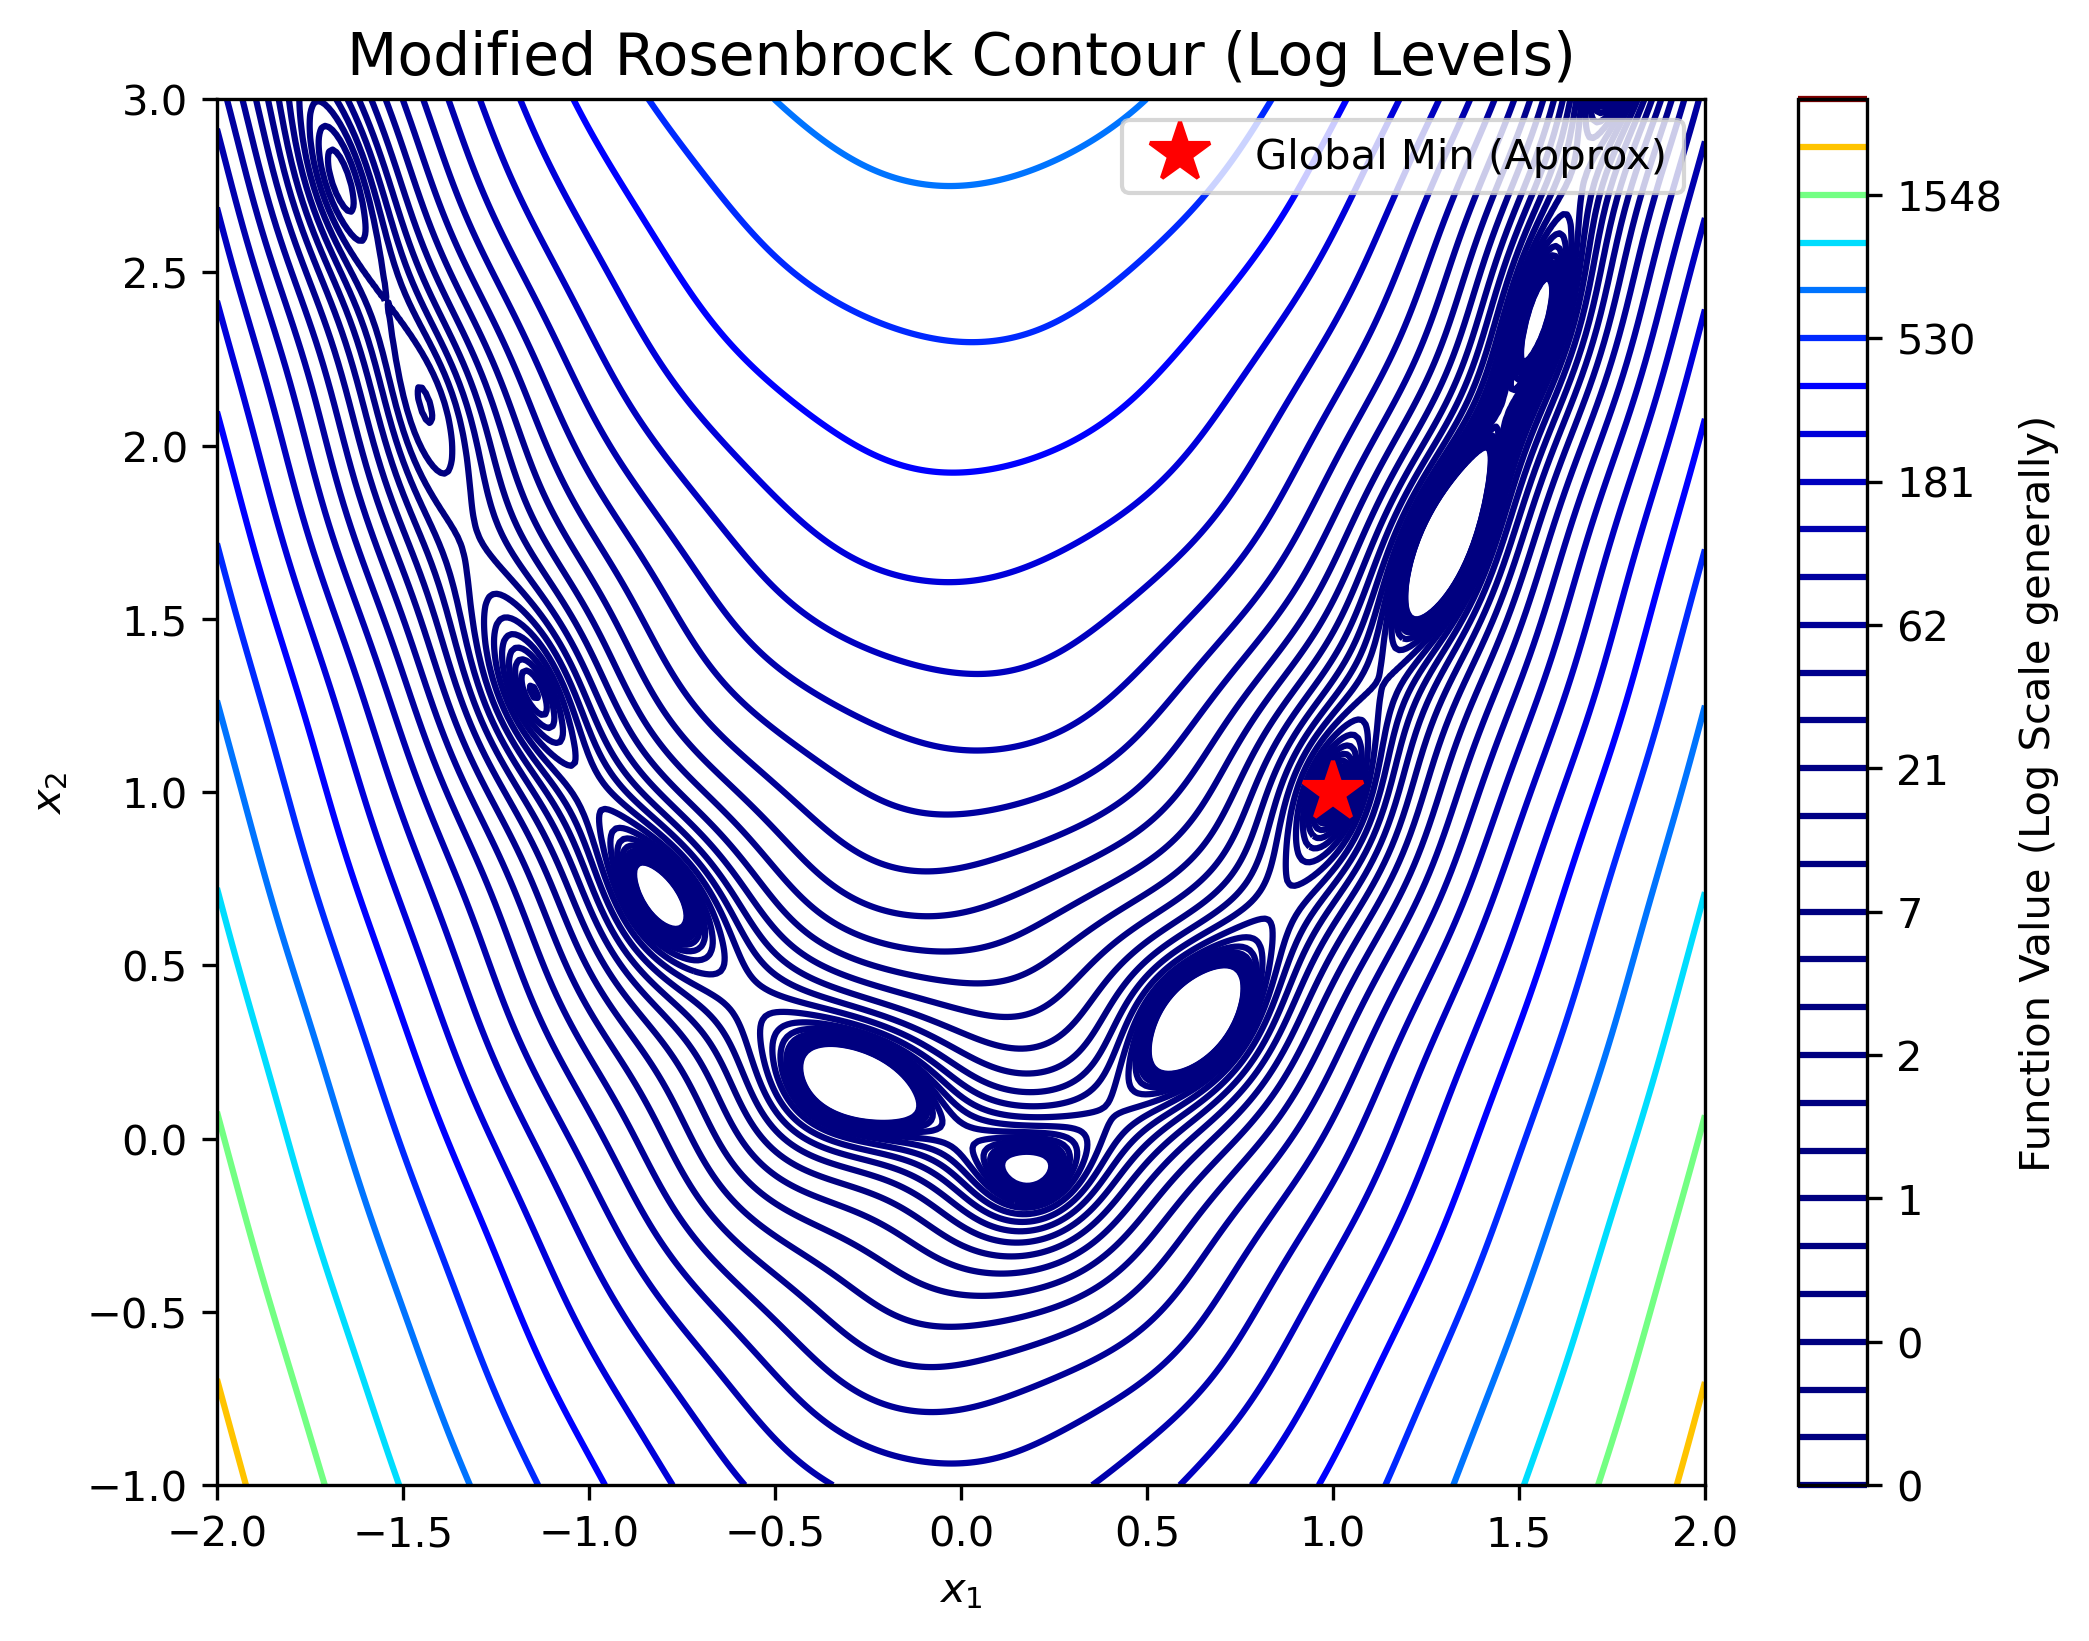
\includegraphics[width=0.8\textwidth]{modified_rosenbrock_contour.png}
    \caption{Modified Rosenbrock 函数等高线图}
    \label{fig:contour}
\end{figure}

\subsection{四维耦合函数——低维 Rosenbrock 扩展版}

\subsubsection{函数定义}
这是一个高维的链式 Rosenbrock 函数，本实验取 $N=4$，表达式为：
\begin{equation}
    f(\bm{x}) = \sum_{k=1}^{3} \left[ (1 - x_k)^2 + 100(x_{k+1} - x_k^2)^2 \right]
\end{equation}

\subsubsection{特性分析}
\begin{itemize}
    \item \textbf{变量耦合与病态性：} 变量之间存在链式依赖关系（$x_{k+1}$ 依赖 $x_k$）。该函数的 Hessian 矩阵在最优解附近条件数极大（Ill-conditioned），导致等高线呈现狭长的“香蕉”形状。对于仅利用一阶梯度的算法（如最速下降法），极易产生“锯齿”现象，收敛速度极慢。
    \item \textbf{高维挑战：} 随着维度增加，搜索空间指数增长，对算法的收敛效率和鲁棒性提出了更高要求。
\end{itemize}


\section{实验原理}
本实验针对无约束优化问题 $\min_{\bm{x} \in \mathbb{R}^n} f(\bm{x})$，本实验实现了基于线搜索（Line Search）和信赖域（Trust Region）两类框架的五种核心算法。
\subsection{线搜索策略}
迭代格式为 $\bm{x}_{k+1} = \bm{x}_k + \alpha_k \bm{d}_k$。本实验对比了两种步长 $\alpha_k$ 的确定方式：

\begin{enumerate}
    \item \textbf{精确线搜索 (Exact Line Search)：}
    通过求解一维极值问题 $\min_{\alpha > 0} \phi(\alpha) = f(\bm{x}_k + \alpha \bm{d}_k)$ 确定步长。
    \item \textbf{非精确线搜索 (Inexact Line Search)：}
    优先尝试满足强 Wolfe 条件 ：

    \begin{gather}
    f(\bm{x}_k + \alpha_k \bm{d}_k) \le f(\bm{x}_k) + c_1 \alpha_k \nabla f(\bm{x}_k)^T \bm{d}_k \quad (\text{Armijo}) \\
    |\nabla f(\bm{x}_k + \alpha_k \bm{d}_k)^T \bm{d}_k| \le c_2 |\nabla f(\bm{x}_k)^T \bm{d}_k| \quad (\text{Curvature})
    \end{gather}
    其中 $c_1=10^{-4}, c_2=0.9$。若无法满足强 Wolfe 条件，代码实现了自动回退机制，使用简单的Armijo回溯法 保证函数值下降。
\end{enumerate}
\subsection{优化算法原理}
\subsubsection{最速下降法 (Steepest Descent)}
利用负梯度方向作为搜索方向，相邻搜索方向正交，收敛速度通常为线性。
\begin{equation}
    d_k = -\nabla f(x_k), \quad x_{k+1} = x_k + \alpha_k d_k
\end{equation}

\subsubsection{牛顿法 (Newton's Method)}
牛顿法利用二阶导数信息（Hessian 矩阵 $\nabla^2 f(\bm{x}_k)$），具有二次收敛速度。但计算代价高，且要求 Hessian 矩阵正定。迭代方向 $\bm{d}_k$ 由下式给出：
\begin{equation}
    \bm{d}_k = -[\nabla^2 f(\bm{x}_k)]^{-1} \bm{g}_k, \quad \bm{x}_{k+1} = \bm{x}_k + \alpha_k \bm{d}_k
\end{equation}
其中 $\bm{g}_k = \nabla f(\bm{x}_k)$ 为梯度。

考虑到目标函数在非凸区域 Hessian 矩阵 $\nabla^2 f(\bm{x}_k)$ 可能非正定或奇异，导致无法求解或方向非下降，此时采用正则化策略（Levenberg-Marquardt 修正）：
\begin{equation}
    (\nabla^2 f(\bm{x}_k) + \epsilon \bm{I}) \bm{d}_k = -\bm{g}_k
\end{equation}
其中 $\epsilon > 0$ 为正则化参数，$\bm{I}$ 为单位矩阵。

\subsubsection{BFGS 拟牛顿法}
BFGS 方法通过迭代更新 Hessian 矩阵的逆矩阵近似 $\bm{H}_k \approx [\nabla^2 f(\bm{x}_k)]^{-1}$，从而避免了直接求逆的计算开销，具有超线性收敛速度。

令 $\bm{s}_k = \bm{x}_{k+1} - \bm{x}_k$ 为位移向量，$\bm{y}_k = \bm{g}_{k+1} - \bm{g}_k$ 为梯度差向量。BFGS 的逆矩阵更新公式如下：
\begin{equation}
    \bm{H}_{k+1} = \left(\bm{I} - \frac{\bm{s}_k \bm{y}_k^T}{\bm{y}_k^T \bm{s}_k}\right) \bm{H}_k \left(\bm{I} - \frac{\bm{y}_k \bm{s}_k^T}{\bm{y}_k^T \bm{s}_k}\right) + \frac{\bm{s}_k \bm{s}_k^T}{\bm{y}_k^T \bm{s}_k}
\end{equation}
此时，搜索方向可以直接通过矩阵乘法计算：$\bm{d}_{k+1} = -\bm{H}_{k+1} \bm{g}_{k+1}$。

\subsubsection{共轭梯度法 (Conjugate Gradient)}

利用共轭方向进行搜索，无需存储矩阵，适合大规模问题。搜索方向构造为 $\bm{d}_k = -\bm{g}_k + \beta_k \bm{d}_{k-1}$。本实验对比了两种公式：
\begin{itemize}
    \item \textbf{FR (Fletcher-Reeves)：} $\beta_k^{FR} = \frac{\|\bm{g}_k\|^2}{\|\bm{g}_{k-1}\|^2}$，理论上对严格凸二次函数收敛，但在非凸问题上可能表现不佳。
    \item \textbf{PRP (Polak-Ribière-Polyak with Restart)：} 
    \begin{equation}
        \beta_k^{PRP} = \frac{\bm{g}_k^T(\bm{g}_k - \bm{g}_{k-1})}{\|\bm{g}_{k-1}\|^2}, \quad \beta_k = \max(0, \beta_k^{PRP})
    \end{equation}
\end{itemize}

\subsubsection{信赖域算法 (Trust Region)}

该算法不进行线搜索，而是维护一个信赖域半径 $\Delta_k$。在每一步，求解子问题：
\begin{equation}
    \min_{\bm{p}} m_k(\bm{p}) = f(\bm{x}_k) + \bm{g}_k^T \bm{p} + \frac{1}{2} \bm{p}^T \bm{H}_k \bm{p}, \quad \text{s.t.} \quad \|\bm{p}\| \le \Delta_k
\end{equation}

本实验采用Dogleg近似求解子问题。Dogleg 路径由两段组成：
\begin{enumerate}
    \item 从原点到柯西点 $\bm{p}^U$（沿负梯度方向的最优点）；
    \item 从柯西点 $\bm{p}^U$ 到牛顿点 $\bm{p}^B$（无约束二次模型极小点 $-\bm{H}^{-1}\bm{g}$）。
\end{enumerate}


\section{参数设置}
\begin{itemize}
    \item \textbf{收敛准则：} 梯度范数 $\|\nabla f(\bm{x}_k)\| \le 10^{-6}$ 或达到最大迭代次数 $k_{max}=1000$。
    \item \textbf{初始点：}
    \begin{itemize}
        \item 2D Modified Rosenbrock: $(-1.2, 1.0)^T$ 等。
        \item 4D Extended Rosenbrock: $(-1.2, 1.0, -0.8, 0.6)^T$ 等。
    \end{itemize}
\end{itemize}


\section{实验内容与结果分析}
\subsection{定量指标对比}

本节展示各算法在不同测试问题及初始点下的收敛性能。主要指标包括迭代次数 ($k$)、最终目标函数值 ($f_{final}$) 以及最终梯度范数 ($\|\bm{g}_{final}\|$)。
本次实验针对两类典型的测试函数：2D Modified Rosenbrock（多极值函数）和 4D Extended Rosenbrock（高维耦合函数），分别测试了最速下降法、牛顿法、BFGS拟牛顿法、共轭梯度法（CG）以及信赖域算法（Trust Region），并对比了精确线搜索与非精确线搜索（Armijo+Wolfe）的效果。

\subsubsection{二维 Modified Rosenbrock 函数}
该函数具有严重的非凸性和大量局部极小值。实验结果如表 \ref{tab:res_2d} 所示。

{
\small % 如果表格太宽，可以用 \small 或 \footnotesize 缩小字体
\setlength{\tabcolsep}{4pt} % 稍微减小列间距以适应页面宽度

\begin{longtable}{llccrrrc}
    % ==========================================
    % 1. 定义表格标题 (Caption)
    % ==========================================
    \caption{2D Modified Rosenbrock 优化结果对比} \label{tab:res_2d} \\

    % ==========================================
    % 2. 定义第一页的表头
    % ==========================================
    \toprule
    \textbf{初始点} & \textbf{算法} & \textbf{策略} & \textbf{迭代次数} & \textbf{时间(s)} & \textbf{$f_{final}$} & \textbf{$\|\bm{g}_{final}\|$} & \textbf{收敛} \\
    \midrule
    \endfirsthead

    % ==========================================
    % 3. 定义后续页面的表头 (自动重复)
    % ==========================================
    \multicolumn{8}{c}{{\bfseries \tablename\ \thetable{} -- 续前页}} \\ % 提示语
    \toprule
    \textbf{初始点} & \textbf{算法} & \textbf{策略} & \textbf{迭代次数} & \textbf{时间(s)} & \textbf{$f_{final}$} & \textbf{$\|\bm{g}_{final}\|$} & \textbf{收敛} \\
    \midrule
    \endhead

    % ==========================================
    % 4. 定义每一页底部的页脚 (可选)
    % ==========================================
    \midrule
    \multicolumn{8}{r}{{接下页...}} \\
    \endfoot

    % ==========================================
    % 5. 定义最后一页底部的页脚 (结束线)
    % ==========================================
    \bottomrule
    \endlastfoot

    % ==========================================
    % 6. 表格正文内容
    % ==========================================
    \multirow{11}{*}{$(-1.2, 1.0)$} 
    & Steepest Descent & Exact & 12 & 0.0044 & -0.9527 & 4.38e-07 & 是 \\
    & Steepest Descent & Inexact & 21 & 0.0060 & 0.8091 & 6.11e-07 & 是 \\
    & Newton & Exact & 5 & 0.0025 & -0.9527 & 4.02e-07 & 是 \\
    & Newton & Inexact & 6 & 0.0020 & -0.9527 & 6.02e-07 & 是 \\
    & BFGS & Exact & 6 & 0.0020 & -0.9527 & 4.74e-07 & 是 \\
    & BFGS & Inexact & 8 & 0.0010 & 0.8091 & 3.05e-09 & 是 \\
    & CG-PRP & Exact & 8 & 0.0031 & -0.9527 & 2.42e-07 & 是 \\
    & CG-PRP & Inexact & 15 & 0.0047 & 0.8091 & 8.33e-07 & 是 \\
    & CG-FP & Exact & 384 & 0.1514 & -1.8506 & 7.41e-07 & 是 \\
    & CG-FP & Inexact & 30 & 0.0094 & 0.8091 & 8.75e-07 & 是 \\
    & Trust Region & TR & 244 & 0.0164 & 4.3378 & 1.68e-07 & 是 \\
    \midrule
    \multirow{11}{*}{$(1.2, 0.5)$} 
    & Steepest Descent & Exact & 30 & 0.0110 & -2.6404 & 9.78e-08 & 是 \\
    & Steepest Descent & Inexact & 28 & 0.0083 & -0.9527 & 9.81e-07 & 是 \\
    & Newton & Exact & 999 & 0.6303 & -0.7183 & 1.26e-06 & 否 \\
    & Newton & Inexact & 5 & 0.0004 & 1.0431 & 4.60e-07 & 是 \\
    & BFGS & Exact & 8 & 0.0024 & 0.8091 & 1.94e-07 & 是 \\
    & BFGS & Inexact & 8 & 0.0010 & 0.8091 & 1.46e-08 & 是 \\
    & CG-PRP & Exact & 999 & 0.5481 & 0.8091 & 1.29e-06 & 否 \\
    & CG-PRP & Inexact & 11 & 0.0031 & 0.8091 & 7.45e-07 & 是 \\
    & CG-FP & Exact & 34 & 0.0129 & -0.9527 & 8.87e-07 & 是 \\
    & CG-FP & Inexact & 13 & 0.0035 & 0.8091 & 6.76e-07 & 是 \\
    & Trust Region & TR & 999 & 0.0544 & 2.4158 & 1.17e-06 & 否 \\
    \midrule
    \multirow{11}{*}{$(-0.5, -0.5)$} 
    & Steepest Descent & Exact & 40 & 0.0129 & 0.0000 & 5.53e-07 & 是 \\
    & Steepest Descent & Inexact & 15 & 0.0038 & -4.5055 & 1.81e-07 & 是 \\
    & Newton & Exact & 6 & 0.0017 & -1.8506 & 4.12e-09 & 是 \\
    & Newton & Inexact & 7 & 0.0008 & -1.8506 & 1.07e-11 & 是 \\
    & BFGS & Exact & 5 & 0.0015 & 0.0000 & 1.52e-09 & 是 \\
    & BFGS & Inexact & 9 & 0.0010 & 0.0000 & 3.90e-07 & 是 \\
    & CG-PRP & Exact & 10 & 0.0042 & -4.5055 & 8.61e-07 & 是 \\
    & CG-PRP & Inexact & 12 & 0.0035 & -4.5055 & 1.64e-09 & 是 \\
    & CG-FP & Exact & 682 & 0.2667 & -4.5055 & 5.53e-07 & 是 \\
    & CG-FP & Inexact & 14 & 0.0041 & 0.0000 & 5.86e-07 & 是 \\
    & Trust Region & TR & 232 & 0.0161 & 2.4158 & 3.32e-08 & 是 \\
    \bottomrule
    \end{longtable}
}

% \begin{table}[H]
% \centering
% \caption{2D Modified Rosenbrock 优化结果对比}
% \label{tab:res_2d}
% \resizebox{\textwidth}{!}{
% \begin{tabular}{llccrrrc}
% \toprule
% \textbf{初始点} & \textbf{算法} & \textbf{策略} & \textbf{迭代次数} & \textbf{时间(s)} & \textbf{$f_{final}$} & \textbf{$\|\bm{g}_{final}\|$} & \textbf{收敛} \\
% \midrule
% \multirow{11}{*}{$(-1.2, 1.0)$} 
%  & Steepest Descent & Exact & 12 & 0.0044 & -0.9527 & 4.38e-07 & 局部极小 \\
%  & Steepest Descent & Inexact & 21 & 0.0060 & 0.8091 & 6.11e-07 & 是 \\
%  & Newton & Exact & 5 & 0.0025 & -0.9527 & 4.02e-07 & 是 \\
%  & Newton & Inexact & 6 & 0.0020 & -0.9527 & 6.02e-07 & 是 \\
%  & BFGS & Exact & 6 & 0.0020 & -0.9527 & 4.74e-07 & 是 \\
%  & BFGS & Inexact & 8 & 0.0010 & 0.8091 & 3.05e-09 & 是 \\
%  & CG-PRP & Exact & 8 & 0.0031 & -0.9527 & 2.42e-07 & 是 \\
%  & CG-PRP & Inexact & 15 & 0.0047 & 0.8091 & 8.33e-07 & 是 \\
%  & CG-FP & Exact & 384 & 0.1514 & -1.8506 & 7.41e-07 & 是 \\
%  & CG-FP & Inexact & 30 & 0.0094 & 0.8091 & 8.75e-07 & 是 \\
%  & Trust Region & TR & 244 & 0.0164 & 4.3378 & 1.68e-07 & 是 \\
% \midrule
% \multirow{11}{*}{$(1.2, 0.5)$} 
%  & Steepest Descent & Exact & 30 & 0.0110 & -2.6404 & 9.78e-08 & 是 \\
%  & Steepest Descent & Inexact & 28 & 0.0083 & -0.9527 & 9.81e-07 & 是 \\
%  & Newton & Exact & 999 & 0.6303 & -0.7183 & 1.26e-06 & 否 \\
%  & Newton & Inexact & 5 & 0.0004 & 1.0431 & 4.60e-07 & 是 \\
%  & BFGS & Exact & 8 & 0.0024 & 0.8091 & 1.94e-07 & 是 \\
%  & BFGS & Inexact & 8 & 0.0010 & 0.8091 & 1.46e-08 & 是 \\
%  & CG-PRP & Exact & 999 & 0.5481 & 0.8091 & 1.29e-06 & 否 \\
%  & CG-PRP & Inexact & 11 & 0.0031 & 0.8091 & 7.45e-07 & 是 \\
%  & CG-FP & Exact & 34 & 0.0129 & -0.9527 & 8.87e-07 & 是 \\
%  & CG-FP & Inexact & 13 & 0.0035 & 0.8091 & 6.76e-07 & 是 \\
%  & Trust Region & TR & 999 & 0.0544 & 2.4158 & 1.17e-06 & 否 \\
% \midrule
% \multirow{11}{*}{$(-0.5, -0.5)$} 
%  & Steepest Descent & Exact & 40 & 0.0129 & 0.0000 & 5.53e-07 & 是 \\
%  & Steepest Descent & Inexact & 15 & 0.0038 & -4.5055 & 1.81e-07 & 是 \\
%  & Newton & Exact & 6 & 0.0017 & -1.8506 & 4.12e-09 & 是 \\
%  & Newton & Inexact & 7 & 0.0008 & -1.8506 & 1.07e-11 & 是 \\
%  & BFGS & Exact & 5 & 0.0015 & 0.0000 & 1.52e-09 & 是 \\
%  & BFGS & Inexact & 9 & 0.0010 & 0.0000 & 3.90e-07 & 是 \\
%  & CG-PRP & Exact & 10 & 0.0042 & -4.5055 & 8.61e-07 & 是 \\
%  & CG-PRP & Inexact & 12 & 0.0035 & -4.5055 & 1.64e-09 & 是 \\
%  & CG-FP & Exact & 682 & 0.2667 & -4.5055 & 5.53e-07 & 是 \\
%  & CG-FP & Inexact & 14 & 0.0041 & 0.0000 & 5.86e-07 & 是 \\
%  & Trust Region & TR & 232 & 0.0161 & 2.4158 & 3.32e-08 & 是 \\
% \bottomrule
% \end{tabular}
% }
% \end{table}
\begin{itemize}
    \item \textbf{多模态陷阱与初值敏感性验证：}
    从表 \ref{tab:res_2d} 可见，不同初始点导致算法收敛到了截然不同的最终函数值 ($f_{final}$)，验证了该函数曲面布满局部极小值：
    \begin{itemize}
        \item 在初始点 $(-1.2, 1.0)$，大多数算法收敛至 $f \approx -0.9527$ 或 $0.8091$。
        \item 在初始点 $(1.2, 0.5)$，部分算法（如 Newton-Exact）甚至未能收敛，而其他算法收敛至局部极小值。
        \item 在初始点 $(-0.5, -0.5)$，Steepest Descent (Inexact) 找到了更优的极小值 $f \approx -4.5055$。
    \end{itemize}
    
    正弦扰动项导致函数地形出现许多“坑洼”。基于梯度的局部搜索算法极易被离初始点最近的局部极小值捕获（Local Minima Traps），难以跳出局部区域寻找全局最优。这表明对于多极值函数，\textbf{初值的选择}起决定性作用。
    
    \item \textbf{信赖域算法 (Trust Region) 的困境：}
    在本实验中，Trust Region 算法在该函数上表现不佳。特别是在 $(-1.2, 1.0)$ 处，迭代 244 次后最终 $f$ 值仍为 4.3378，远差于其他算法。这是因为信赖域算法通常基于局部二次模型（Quadratic Model）来近似目标函数。由于 Modified Rosenbrock 叠加了剧烈震荡的正弦波，导致局部二次近似在稍大的信赖域半径内失效，算法被迫反复缩小半径，导致迭代停滞或进展极慢。
    \item \textbf{收敛速度对比：}
    尽管面临多极值困难，\textbf{牛顿法和 BFGS} 在成功收敛的情况下依然表现出极快的速度（通常迭代次数 $< 10$），体现了二阶信息在局部寻优中的高效性。
\end{itemize}


\subsubsection{四维 Extended Rosenbrock 函数}
该函数主要考察算法处理高维病态（Ill-conditioned）问题的能力。结果如表 \ref{tab:res_4d} 所示。

{
\small % 如果表格太宽，可以用 \small 或 \footnotesize 缩小字体
\setlength{\tabcolsep}{4pt} % 稍微减小列间距以适应页面宽度

\begin{longtable}{llccrrrc}
    % ==========================================
    % 1. 定义表格标题 (Caption)
    % ==========================================
    \caption{4D Modified Rosenbrock 优化结果对比} \label{tab:res_4d} \\

    % ==========================================
    % 2. 定义第一页的表头
    % ==========================================
    \toprule
    \textbf{初始点} & \textbf{算法} & \textbf{策略} & \textbf{迭代次数} & \textbf{时间(s)} & \textbf{$f_{final}$} & \textbf{$\|\bm{g}_{final}\|$} & \textbf{收敛} \\
    \midrule
    \endfirsthead

    % ==========================================
    % 3. 定义后续页面的表头 (自动重复)
    % ==========================================
    \multicolumn{8}{c}{{\bfseries \tablename\ \thetable{} -- 续前页}} \\ % 提示语
    \toprule
    \textbf{初始点} & \textbf{算法} & \textbf{策略} & \textbf{迭代次数} & \textbf{时间(s)} & \textbf{$f_{final}$} & \textbf{$\|\bm{g}_{final}\|$} & \textbf{收敛} \\
    \midrule
    \endhead

    % ==========================================
    % 4. 定义每一页底部的页脚 (可选)
    % ==========================================
    \midrule
    \multicolumn{8}{r}{{接下页...}} \\
    \endfoot

    % ==========================================
    % 5. 定义最后一页底部的页脚 (结束线)
    % ==========================================
    \bottomrule
    \endlastfoot

    % ==========================================
    % 6. 表格正文内容
    % ==========================================
    \multirow{11}{*}{$(-1.2, 1.0, -0.8, 0.6)$} 
    & Steepest Descent & Exact & 999 & 0.2877 & 0.0149 & 1.46e-01 & 否 \\
    & Steepest Descent & Inexact & 999 & 0.2754 & 0.0362 & 3.19e-01 & 否 \\
    & Newton & Exact & 11 & 0.0035 & 3.7014 & 1.56e-07 & 是 \\
    & Newton & Inexact & 9 & 0.0008 & 3.7014 & 9.44e-11 & 是 \\
    & BFGS & Exact & 27 & 0.0082 & 0.0000 & 1.50e-08 & 是 \\
    & BFGS & Inexact & 47 & 0.0052 & 0.0000 & 3.77e-07 & 是 \\
    & CG-PRP & Exact & 999 & 0.3654 & 0.0000 & 1.76e-06 & 否 \\
    & CG-PRP & Inexact & 79 & 0.0216 & 0.0000 & 5.68e-07 & 是 \\
    & CG-FP & Exact & 999 & 0.3873 & 0.0000 & 3.36e-06 & 否 \\
    & CG-FP & Inexact & 999 & 0.4420 & 0.0465 & 3.95e+00 & 否 \\
    & Trust Region & TR & 999 & 0.0660 & 130.0445 & 2.96e+02 & 否 \\
    \midrule
    \multirow{11}{*}{$(0, 0, 0, 0)$} 
    & Steepest Descent & Exact & 999 & 0.2664 & 0.0069 & 2.37e-01 & 否 \\
    & Steepest Descent & Inexact & 999 & 0.2601 & 0.0238 & 3.62e-01 & 否 \\
    & Newton & Exact & 12 & 0.0032 & 0.0000 & 9.15e-08 & 是 \\
    & Newton & Inexact & 16 & 0.0014 & 0.0000 & 9.22e-08 & 是 \\
    & BFGS & Exact & 27 & 0.0073 & 0.0000 & 4.60e-07 & 是 \\
    & BFGS & Inexact & 34 & 0.0035 & 0.0000 & 2.34e-07 & 是 \\
    & CG-PRP & Exact & 969 & 0.3383 & 0.0000 & 9.99e-07 & 是 \\
    & CG-PRP & Inexact & 54 & 0.0127 & 0.0000 & 3.12e-07 & 是 \\
    & CG-FP & Exact & 999 & 0.3077 & 0.0000 & 9.02e-06 & 否 \\
    & CG-FP & Inexact & 999 & 0.3281 & 0.0000 & 2.82e-06 & 否 \\
    & Trust Region & TR & 100 & 0.0061 & 0.0000 & 8.56e-09 & 是 \\
    \midrule
    \multirow{11}{*}{$(-1, -1, -1, -1)$} 
    & Steepest Descent & Exact & 999 & 0.2701 & 0.0346 & 2.62e-01 & 否 \\
    & Steepest Descent & Inexact & 999 & 0.3167 & 0.0380 & 3.08e-01 & 否 \\
    & Newton & Exact & 17 & 0.0063 & 0.0000 & 2.78e-08 & 是 \\
    & Newton & Inexact & 22 & 0.0027 & 0.0000 & 3.95e-08 & 是 \\
    & BFGS & Exact & 32 & 0.0113 & 0.0000 & 8.25e-08 & 是 \\
    & BFGS & Inexact & 24 & 0.0028 & 0.0000 & 8.35e-08 & 是 \\
    & CG-PRP & Exact & 372 & 0.1300 & 0.0000 & 9.04e-07 & 是 \\
    & CG-PRP & Inexact & 792 & 0.2649 & 0.0000 & 1.00e-06 & 是 \\
    & CG-FP & Exact & 999 & 0.3495 & 0.9184 & 4.87e+01 & 否 \\
    & CG-FP & Inexact & 999 & 0.4706 & 0.0070 & 1.01e+00 & 否 \\
    & Trust Region & TR & 999 & 0.0666 & 620.6691 & 1.16e+03 & 否 \\
\end{longtable}
}
% \begin{table}[H]
% \centering
% \caption{4D Extended Rosenbrock 优化结果对比}
% \label{tab:res_4d}
% \resizebox{\textwidth}{!}{
% \begin{tabular}{llccrrrc}
% \toprule
% \textbf{初始点} & \textbf{算法} & \textbf{策略} & \textbf{迭代次数} & \textbf{时间(s)} & \textbf{$f_{final}$} & \textbf{$\|\bm{g}_{final}\|$} & \textbf{收敛} \\
% \midrule
% \multirow{11}{*}{$(-1.2, 1.0, -0.8, 0.6)$} 
%  & Steepest Descent & Exact & 999 & 0.2877 & 0.0149 & 1.46e-01 & 否 \\
%  & Steepest Descent & Inexact & 999 & 0.2754 & 0.0362 & 3.19e-01 & 否 \\
%  & Newton & Exact & 11 & 0.0035 & 3.7014 & 1.56e-07 & 是 \\
%  & Newton & Inexact & 9 & 0.0008 & 3.7014 & 9.44e-11 & 是 \\
%  & BFGS & Exact & 27 & 0.0082 & 0.0000 & 1.50e-08 & 是 \\
%  & BFGS & Inexact & 47 & 0.0052 & 0.0000 & 3.77e-07 & 是 \\
%  & CG-PRP & Exact & 999 & 0.3654 & 0.0000 & 1.76e-06 & 否 \\
%  & CG-PRP & Inexact & 79 & 0.0216 & 0.0000 & 5.68e-07 & 是 \\
%  & CG-FP & Exact & 999 & 0.3873 & 0.0000 & 3.36e-06 & 否 \\
%  & CG-FP & Inexact & 999 & 0.4420 & 0.0465 & 3.95e+00 & 否 \\
%  & Trust Region & TR & 999 & 0.0660 & 130.0445 & 2.96e+02 & 否 \\
% \midrule
% \multirow{11}{*}{$(0, 0, 0, 0)$} 
%  & Steepest Descent & Exact & 999 & 0.2664 & 0.0069 & 2.37e-01 & 否 \\
%  & Steepest Descent & Inexact & 999 & 0.2601 & 0.0238 & 3.62e-01 & 否 \\
%  & Newton & Exact & 12 & 0.0032 & 0.0000 & 9.15e-08 & 是 \\
%  & Newton & Inexact & 16 & 0.0014 & 0.0000 & 9.22e-08 & 是 \\
%  & BFGS & Exact & 27 & 0.0073 & 0.0000 & 4.60e-07 & 是 \\
%  & BFGS & Inexact & 34 & 0.0035 & 0.0000 & 2.34e-07 & 是 \\
%  & CG-PRP & Exact & 969 & 0.3383 & 0.0000 & 9.99e-07 & 是 \\
%  & CG-PRP & Inexact & 54 & 0.0127 & 0.0000 & 3.12e-07 & 是 \\
%  & CG-FP & Exact & 999 & 0.3077 & 0.0000 & 9.02e-06 & 否 \\
%  & CG-FP & Inexact & 999 & 0.3281 & 0.0000 & 2.82e-06 & 否 \\
%  & Trust Region & TR & 100 & 0.0061 & 0.0000 & 8.56e-09 & 是 \\
% \midrule
% \multirow{11}{*}{$(-1, -1, -1, -1)$} 
%  & Steepest Descent & Exact & 999 & 0.2701 & 0.0346 & 2.62e-01 & 否 \\
%  & Steepest Descent & Inexact & 999 & 0.3167 & 0.0380 & 3.08e-01 & 否 \\
%  & Newton & Exact & 17 & 0.0063 & 0.0000 & 2.78e-08 & 是 \\
%  & Newton & Inexact & 22 & 0.0027 & 0.0000 & 3.95e-08 & 是 \\
%  & BFGS & Exact & 32 & 0.0113 & 0.0000 & 8.25e-08 & 是 \\
%  & BFGS & Inexact & 24 & 0.0028 & 0.0000 & 8.35e-08 & 是 \\
%  & CG-PRP & Exact & 372 & 0.1300 & 0.0000 & 9.04e-07 & 是 \\
%  & CG-PRP & Inexact & 792 & 0.2649 & 0.0000 & 1.00e-06 & 是 \\
%  & CG-FP & Exact & 999 & 0.3495 & 0.9184 & 4.87e+01 & 否 \\
%  & CG-FP & Inexact & 999 & 0.4706 & 0.0070 & 1.01e+00 & 否 \\
%  & Trust Region & TR & 999 & 0.0666 & 620.6691 & 1.16e+03 & 否 \\
% \bottomrule
% \end{tabular}
% }
% \end{table}




\begin{itemize}
    \item \textbf{最速下降法的失效：} 在所有 4D 测试中，最速下降法（Steepest Descent）均未能在 1000 次迭代内达到 $10^{-6}$ 的收敛精度。这是因为 Rosenbrock 函数具有狭长的弯曲山谷结构，梯度方向与指向极小值点的方向几乎垂直，导致算法在谷底呈“之”字形锯齿状震荡，步长极小但无法有效向前推进。
    \item \textbf{二阶/拟牛顿法的鲁棒性：} BFGS 和 Newton 法表现优异，这证明了利用二阶曲率信息（或其近似）对于解决病态问题至关重要。特别是 BFGS，在 $(-1.2, 1.,-0.8, 0.6)$ 中成功找到了全局极小值 0.0000，而 Newton 法陷入了局部极小值 3.7014。这说明 BFGS 通过历史梯度信息构建的 Hessian 近似矩阵，在某种程度上比纯粹的局部二阶信息更具鲁棒性。
    \item \textbf{精确 vs 非精确线搜索}：从时间上看，非精确线搜索（Inexact）通常比精确线搜索（Exact）更耗时少（例如牛顿法 0.0008s vs 0.003s），且往往能以更少的步数收敛，因为精确搜索在每一步过度优化可能会导致后续搜索方向偏离全局最优路径。
\end{itemize}



\subsection{定性结果可视化}

\subsubsection{收敛曲线分析}

图 \ref{fig:conv_curves} 展示了不同算法在优化过程中梯度范数 $\log_{10}(\|\bm{g}\|)$ 随迭代次数的变化情况，直观地反映了各算法的收敛性质：
% \begin{figure}[H]
%     \centering
%     % 第一张图：2D
%     \subfloat[2D Modified Rosenbrock 收敛曲线]{
%         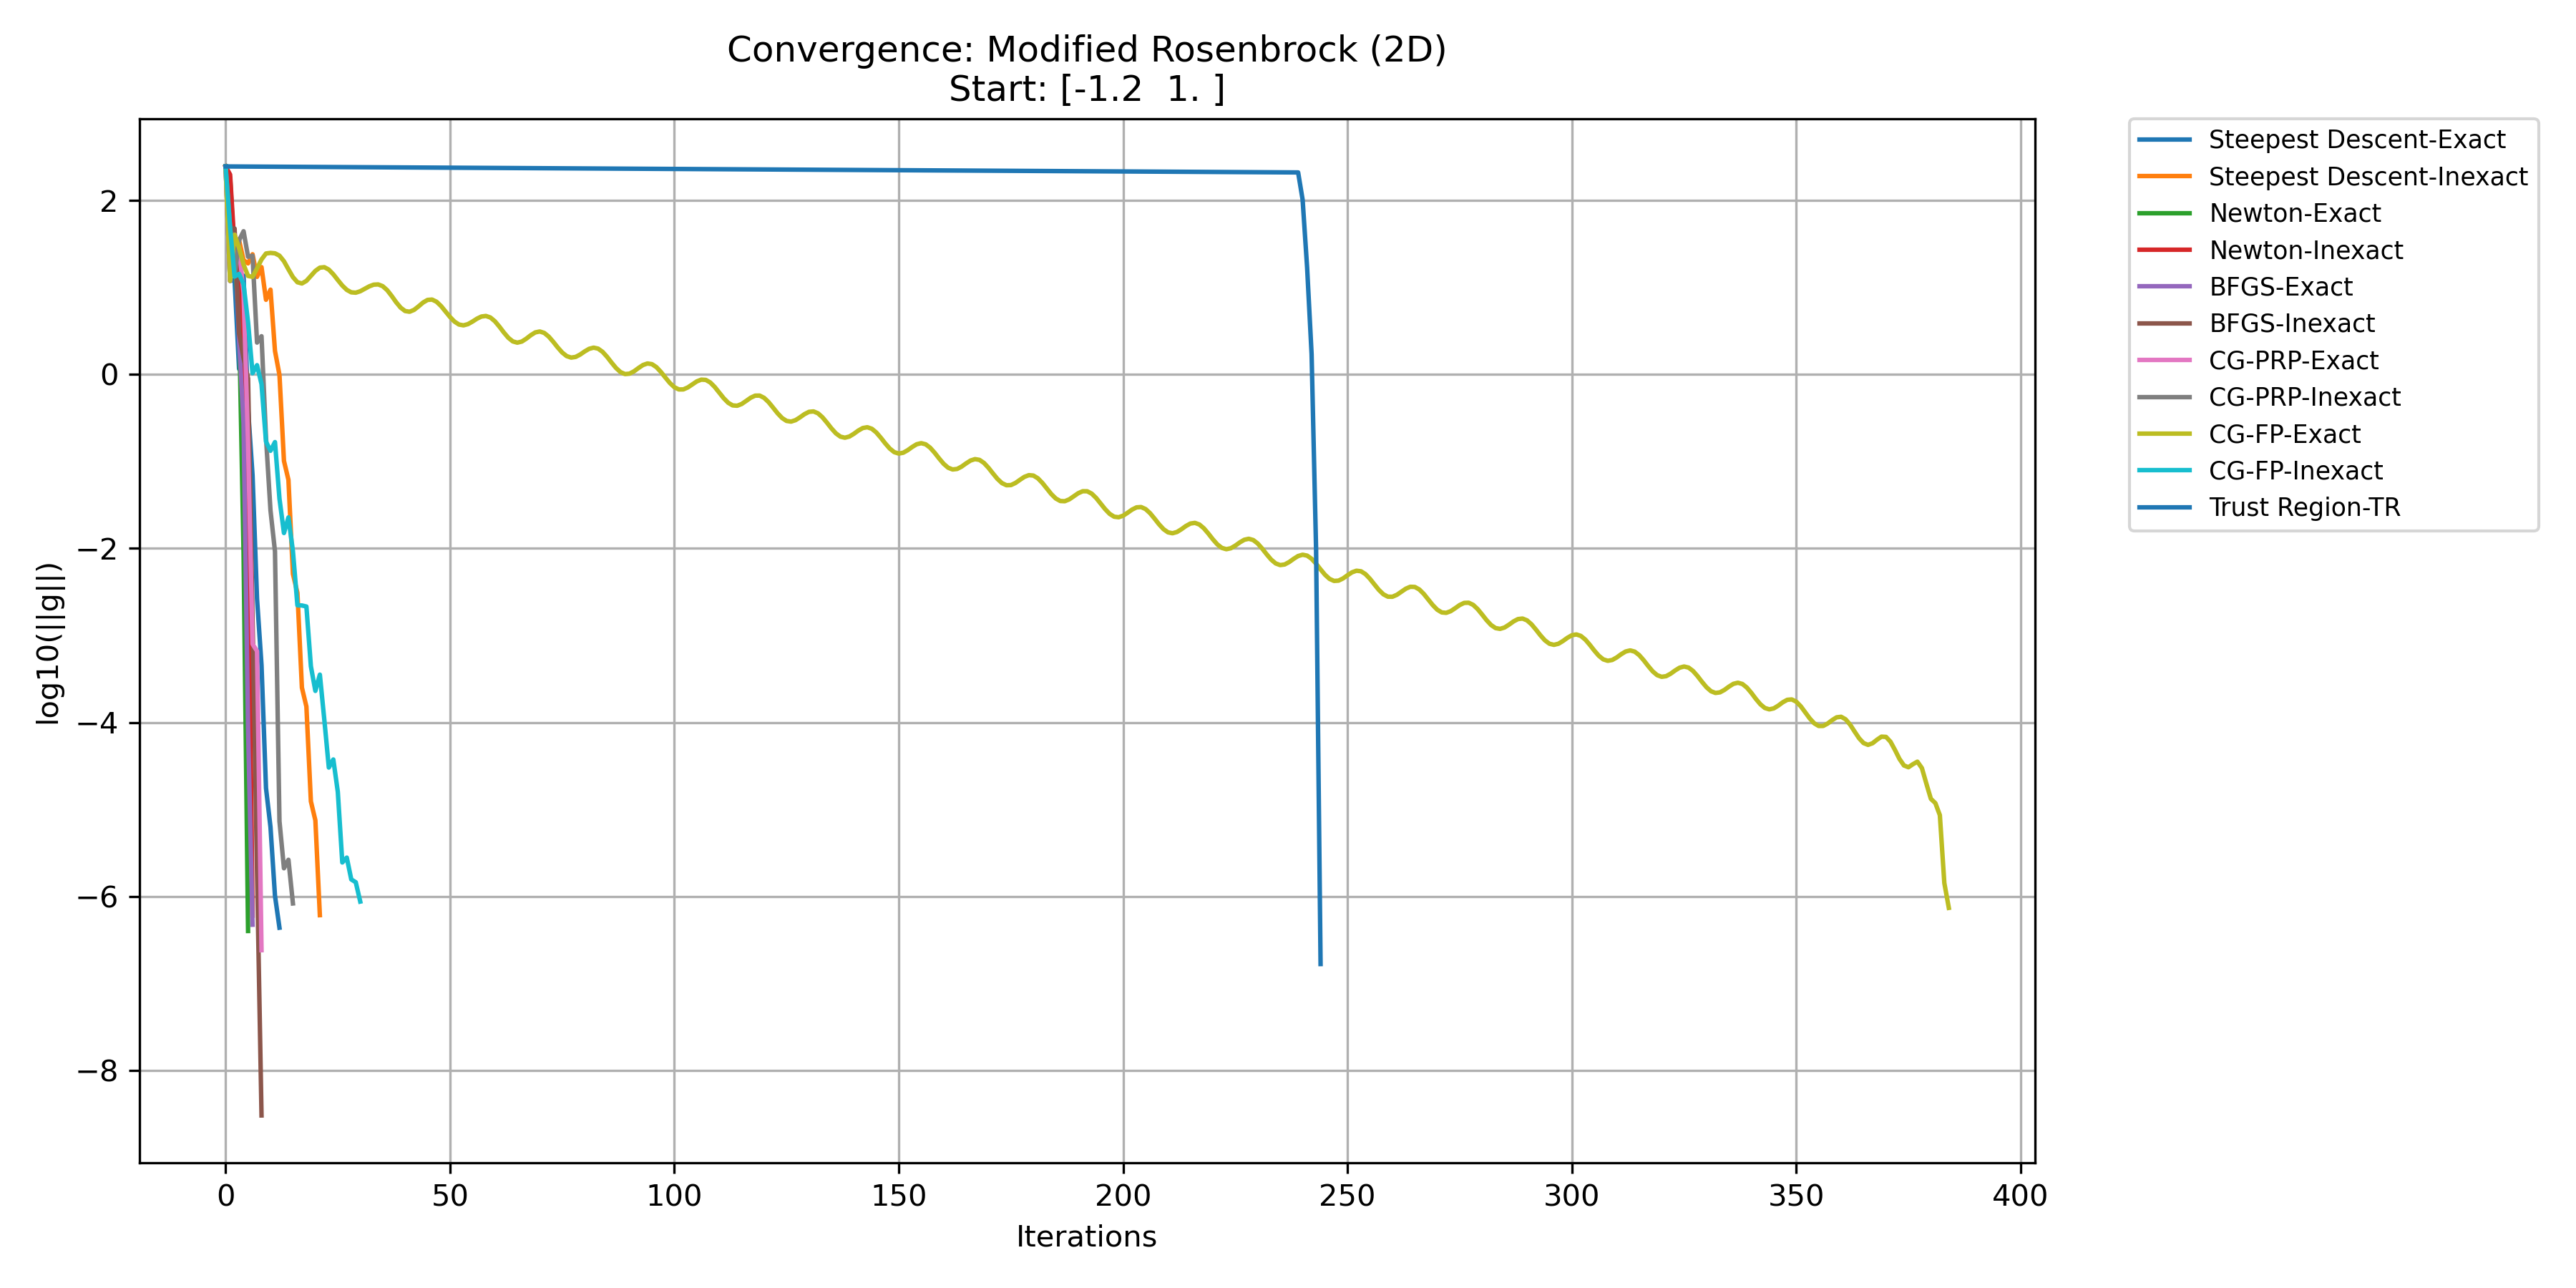
\includegraphics[width=0.8\textwidth]{convergence_plot_2d.png}}
%     \\ 
%     % 第二张图：4D
%     \subfloat[4D Extended Rosenbrock 收敛曲线]{
%         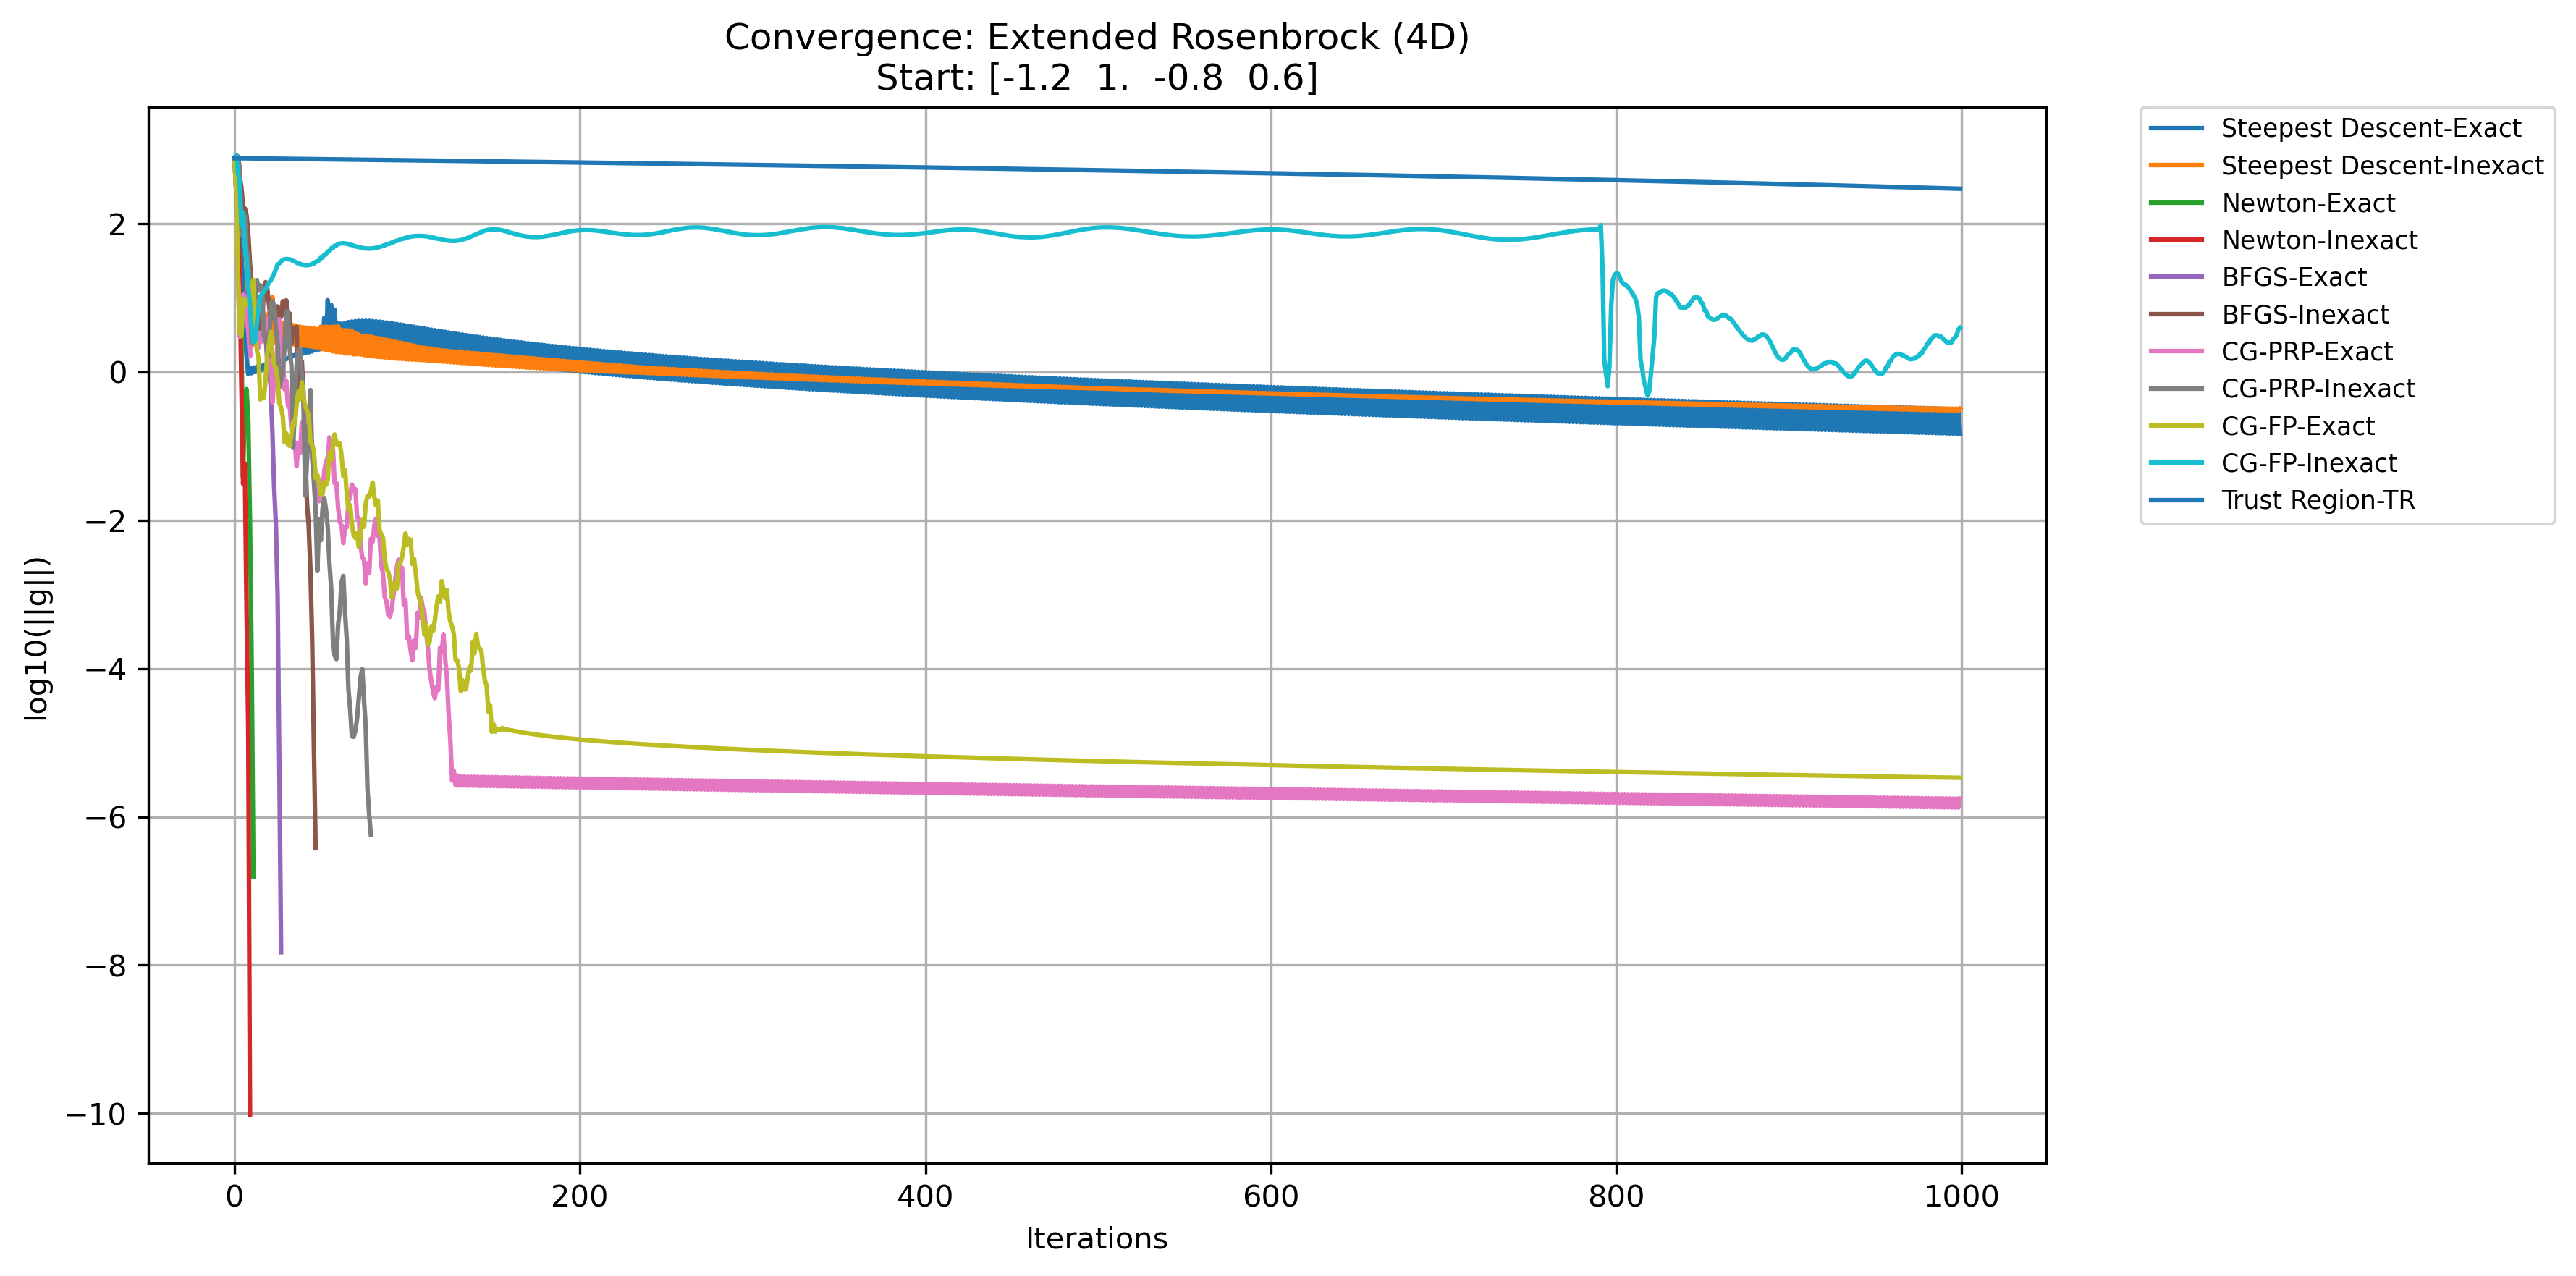
\includegraphics[width=0.8\textwidth]{convergence_plot_4d.png}}
%     \caption{各算法收敛速度对比}
%     \label{fig:conv_curves}
% \end{figure}

\begin{figure}[H]
    \centering
    \setcounter{subfigure}{0} % 重置子图计数器
    % 子图 A
    % \subfloat[子标题]{图片命令}
    \subfloat[2D Modified Rosenbrock 收敛曲线]{
        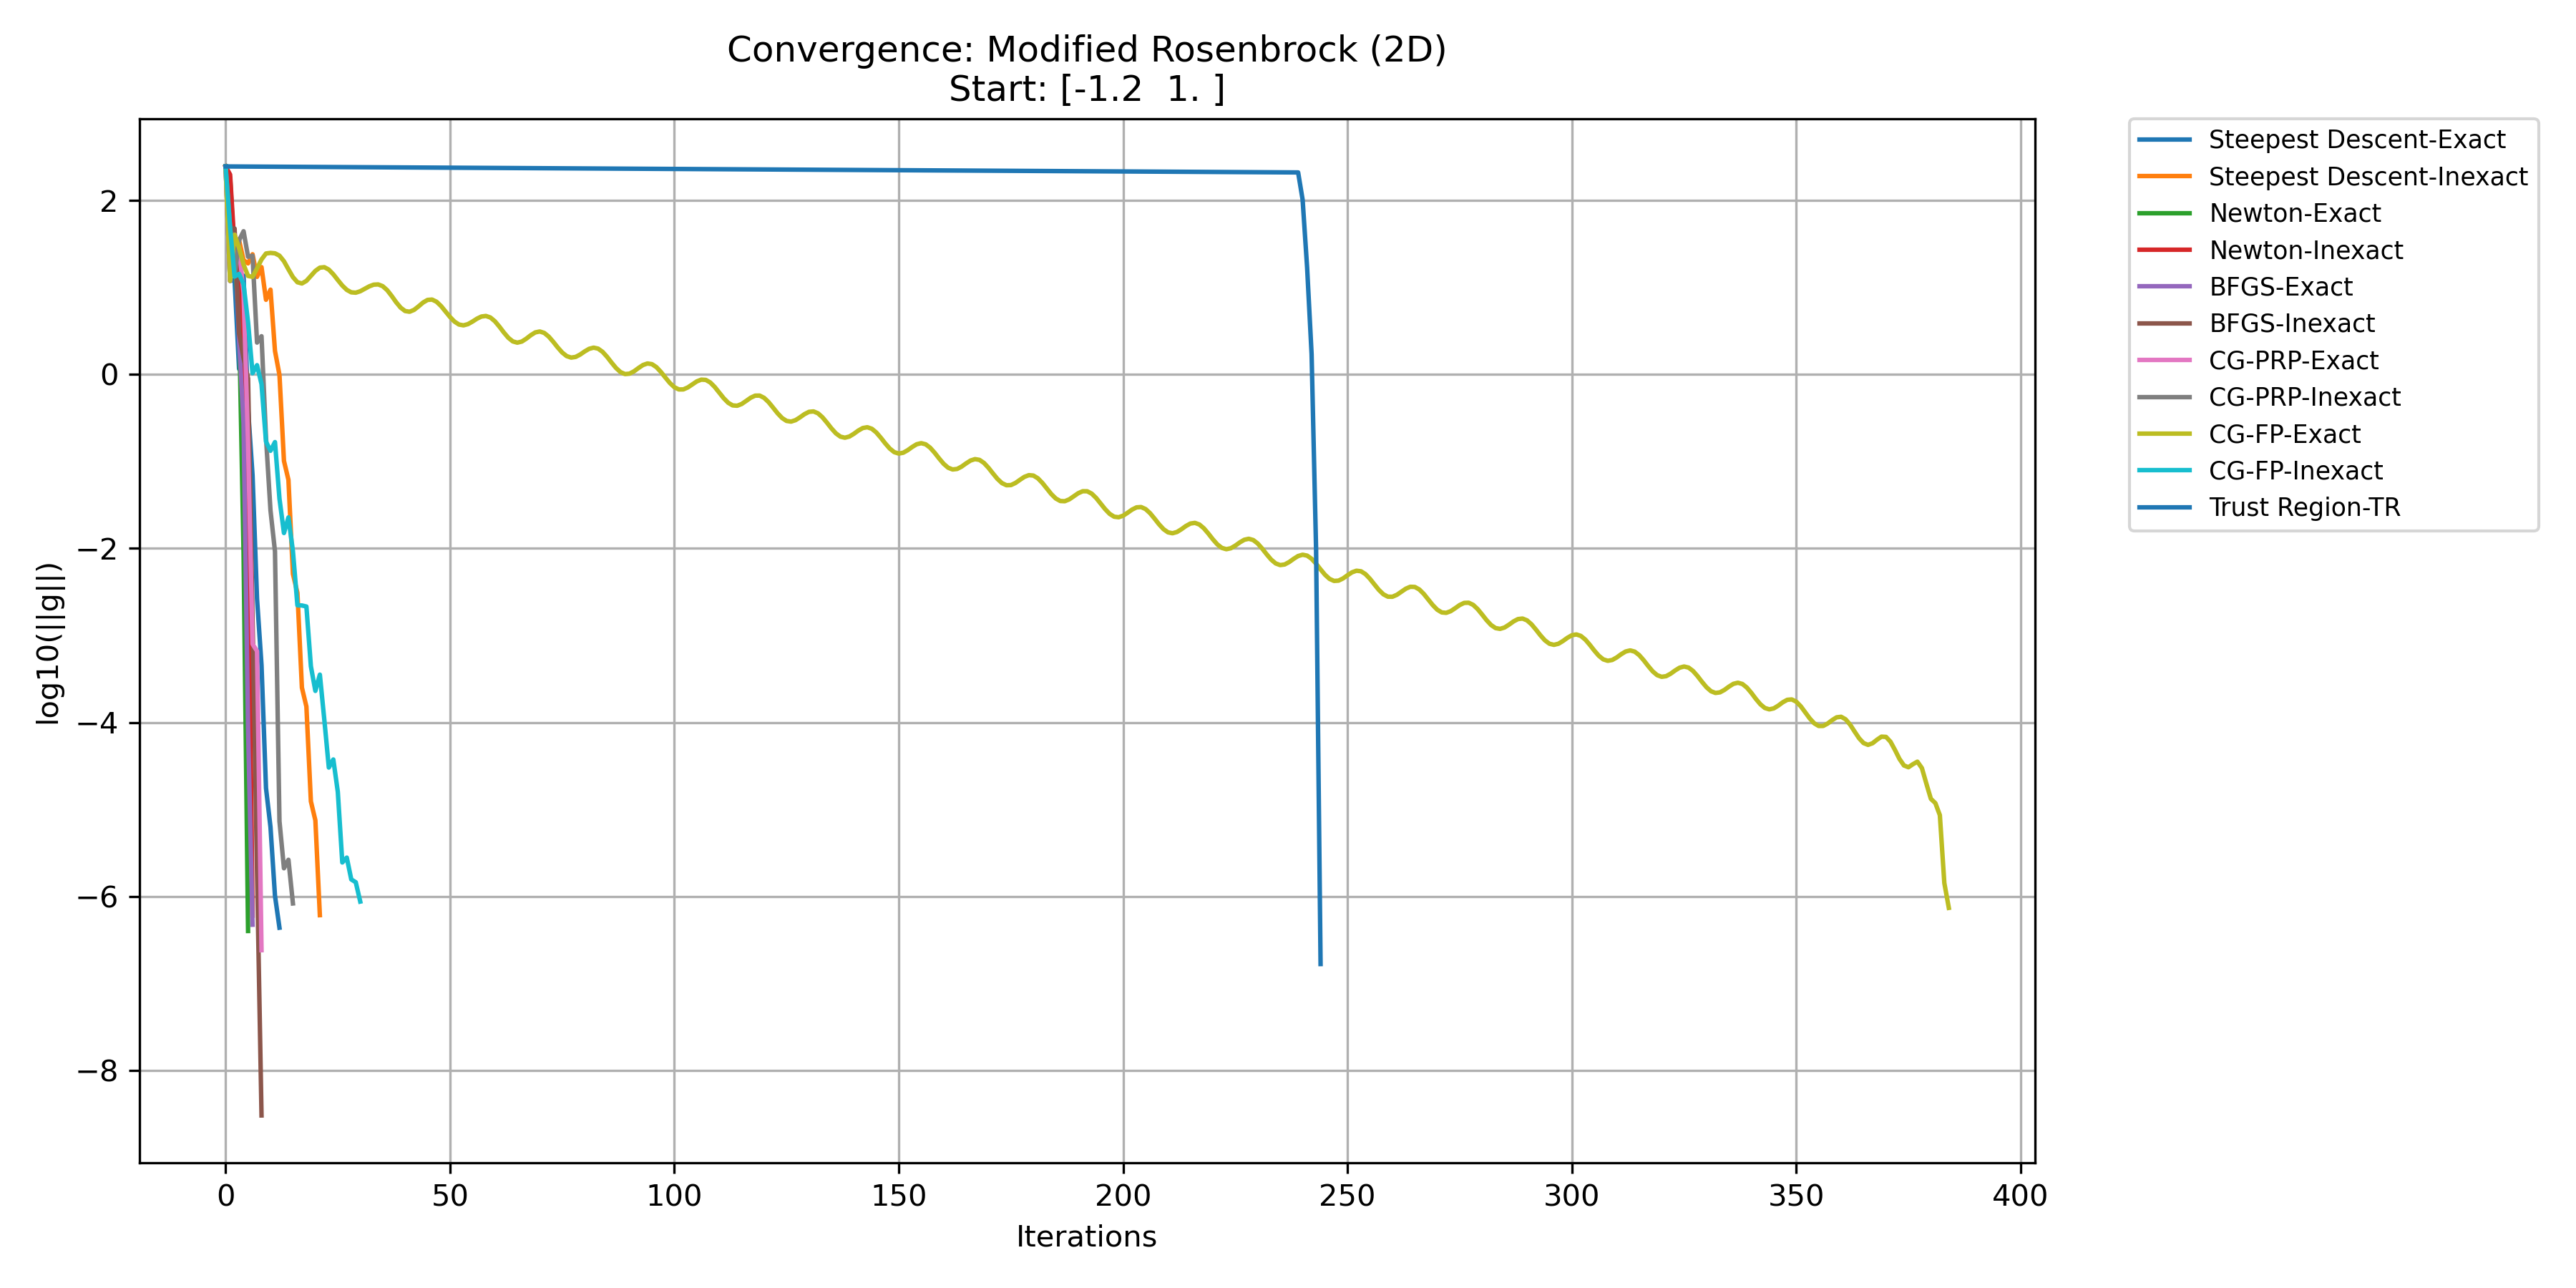
\includegraphics[width=1\linewidth]{convergence_plot_2d.png}
    }
    
    % 【关键点 1】总标题放在第一部分
    \caption{无约束优化收敛曲线对比}
    
    % 【关键点 2】Label 放在第一部分，这样 \ref{fig:conv_curves} 会指向图 1
    \label{fig:conv_curves} 
\end{figure}

% --- 强制分页 ---
\clearpage

% --- 第二部分：图 1(b) 所在页 ---
\begin{figure}[H]
    % 【关键点 3】告诉 LaTeX 接续上一张图的编号
    \ContinuedFloat 
    \centering
    
    % 子图 B
    \subfloat[4D Extended Rosenbrock 收敛曲线]{
        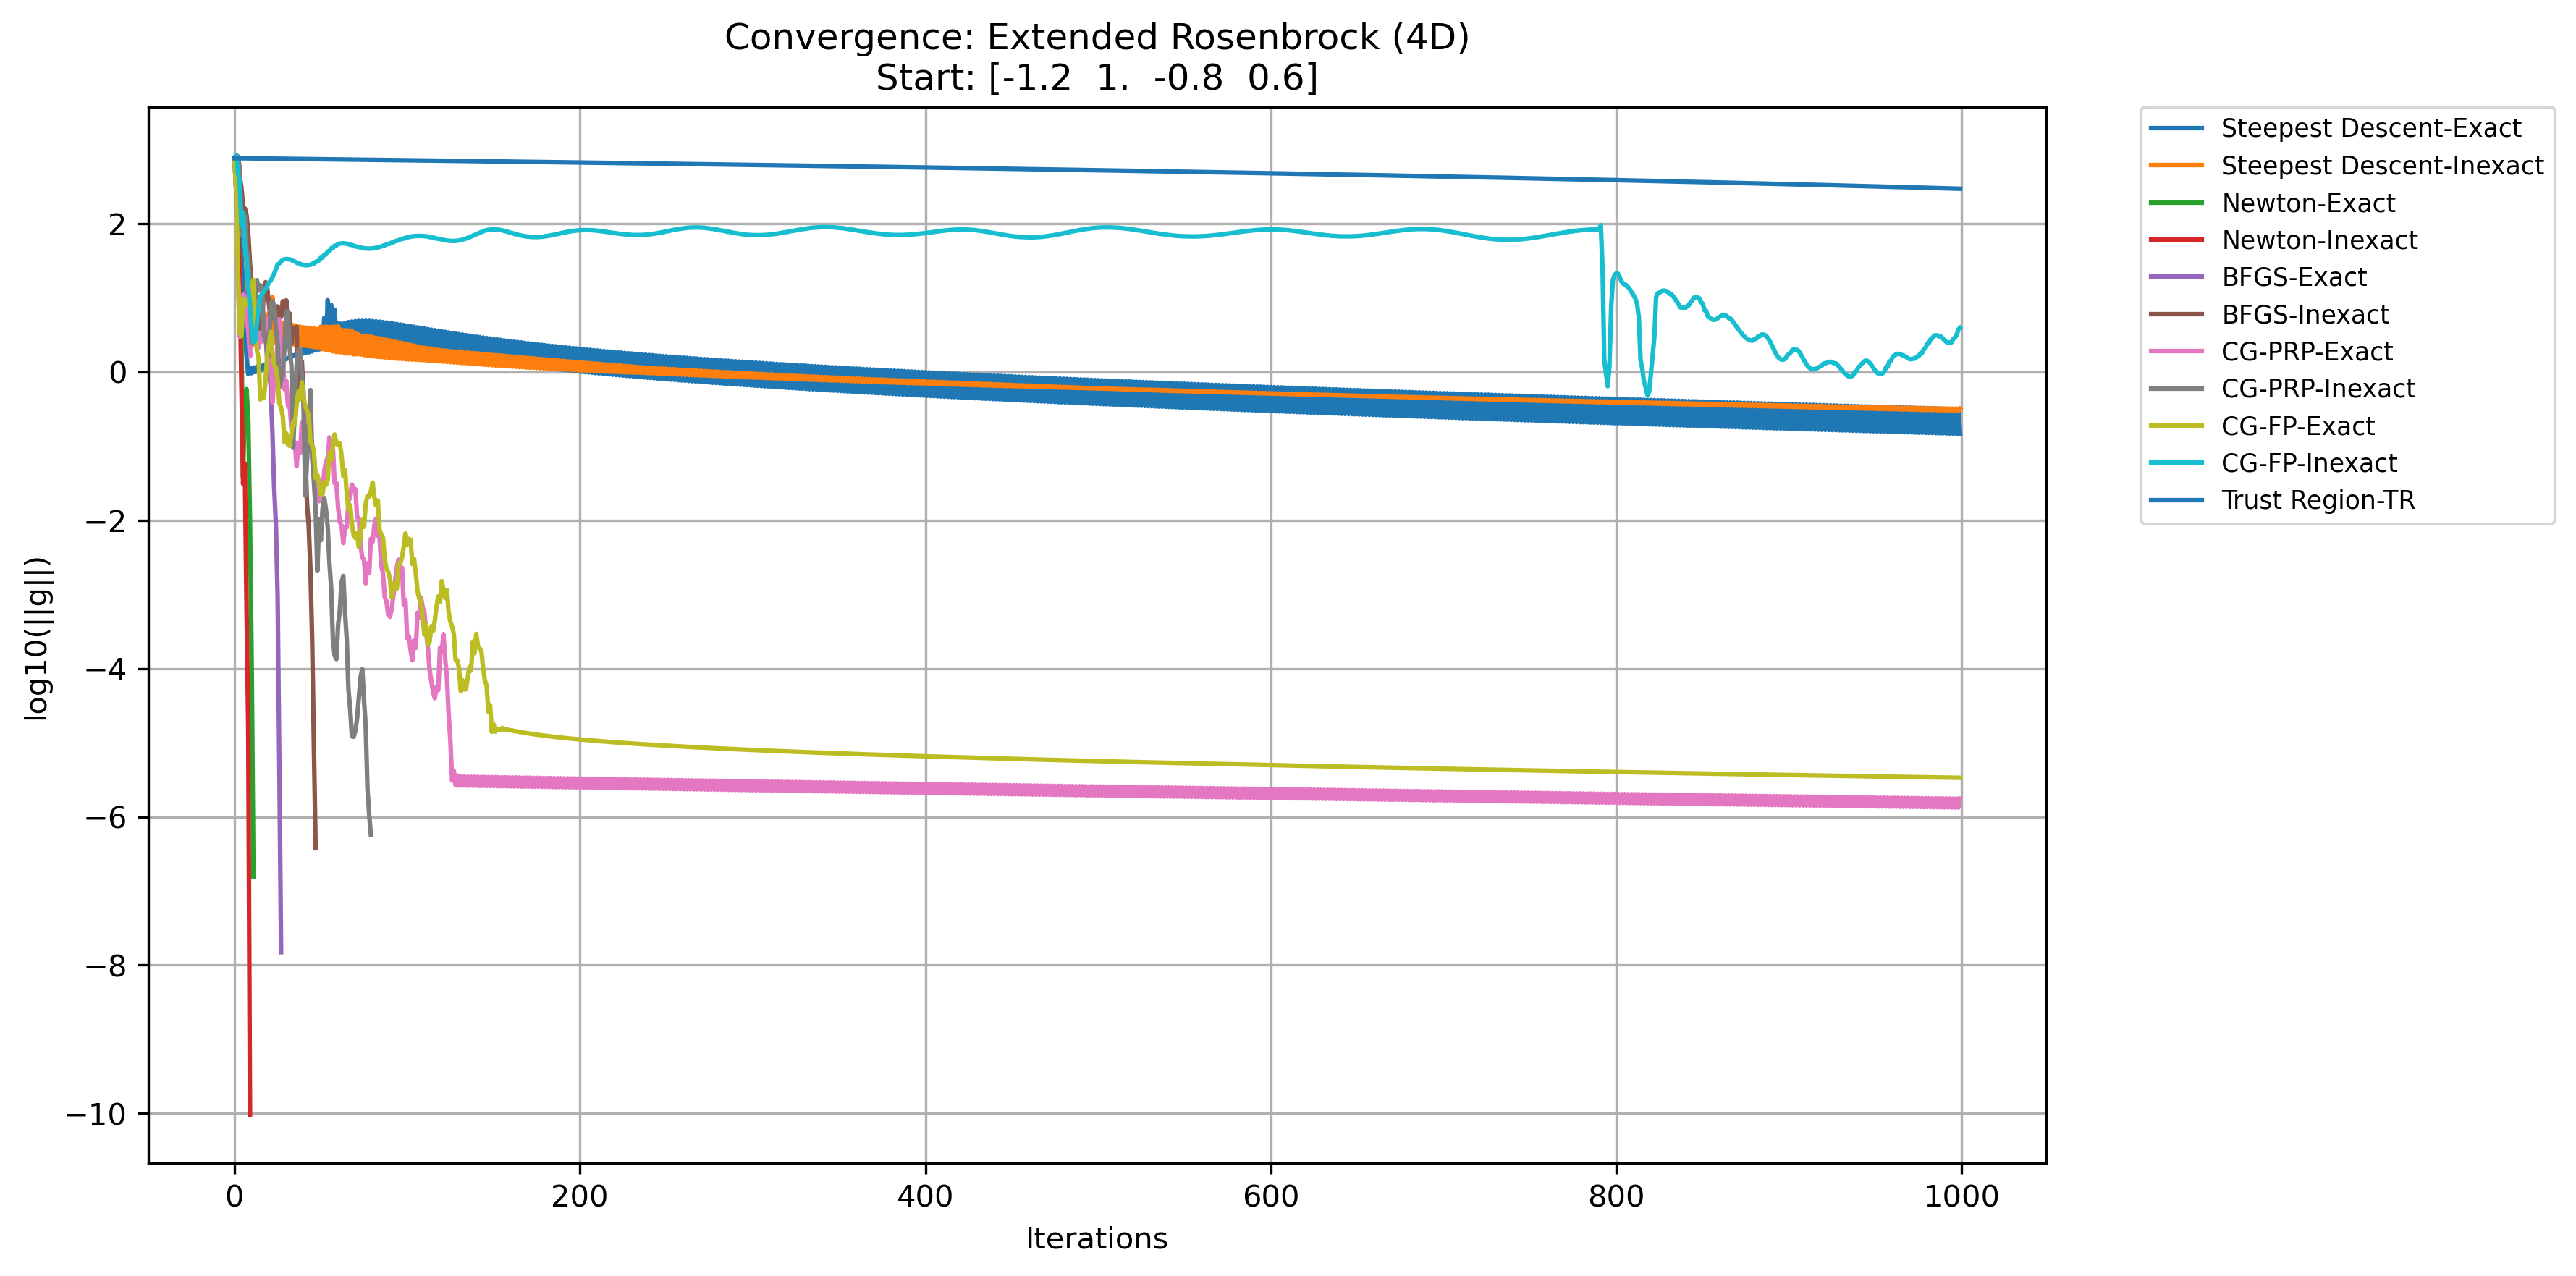
\includegraphics[width=1\linewidth]{convergence_plot_4d.png}
    }
    
    % 这里通常写一个续表标题，或者空的 [] 避免生成多余的目录项
    \caption[]{无约束优化收敛曲线对比（续）} 
\end{figure}

从图中清晰可见，\textbf{最速下降法}（图中的橙色/蓝色平缓线）的收敛速率仅为线性，曲线下降非常缓慢，甚至在长时间迭代后仍停留在较高误差水平。

相比之下，\textbf{Newton 法和 BFGS 算法}（绿色/紫色线）呈现出典型的超线性或二阶收敛特征。在通过初期的调整后，梯度范数在接近最优解时出现“断崖式”下跌（Cliff-like drop），仅需极少的迭代次数即可达到机器精度。

\paragraph{2D Modified Rosenbrock 的地形影响（子图a）}
该图中 \textbf{CG-FP-Exact}（黄线）呈现出显著的周期性震荡轨迹。这直观地反映了算法在应对由正弦项 $5\sin(2\pi x_i)$  引入的\textbf{密集局部极值地貌}时的搜索行为。轨迹的每一次起伏都对应着算法在局部凸凹结构之间的穿越与调整。而信赖域算法（深蓝线）前期的长时间平滞则表明其陷入了某个非最优的局部平稳点。
\paragraph{4D Extended Rosenbrock 的病态特征（子图b）}
该图最显著的特征是 \textbf{最速下降法} 近乎水平的直线，这揭示了 Rosenbrock 函数著名的“香蕉谷”病态地形导致的\textbf{锯齿效应（Zig-zagging）}——负梯度方向与峡谷延伸方向垂直，导致算法在谷壁间反复震荡却无法前行。而 \textbf{CG-FP-Inexact}（青色线）后期的剧烈震荡发散，则说明了非精确线搜索在高维病态问题中容易导致共轭梯度法的方向共轭性失效。


\subsubsection{搜索路径分析}

图 \ref{fig:opt_paths} 直观地展示了各算法在 2D Modified Rosenbrock 函数等高线图上的搜索轨迹。该函数的最大特征在于其抛物线山谷中叠加了高频正弦波纹，形成了密集的局部极小值陷阱（Local Minima Traps）。从图中可见，所有算法均未能从初始点 $(-1.2, 1.0)$ 成功抵达全局极小值 $(1, 1)$，而是分别陷入了不同的局部吸引域中。
\begin{figure}[H]
    \setcounter{subfigure}{0}
    \centering
    \subfloat[2D Modified Rosenbrock 优化路径 (Inexact Search)]{
        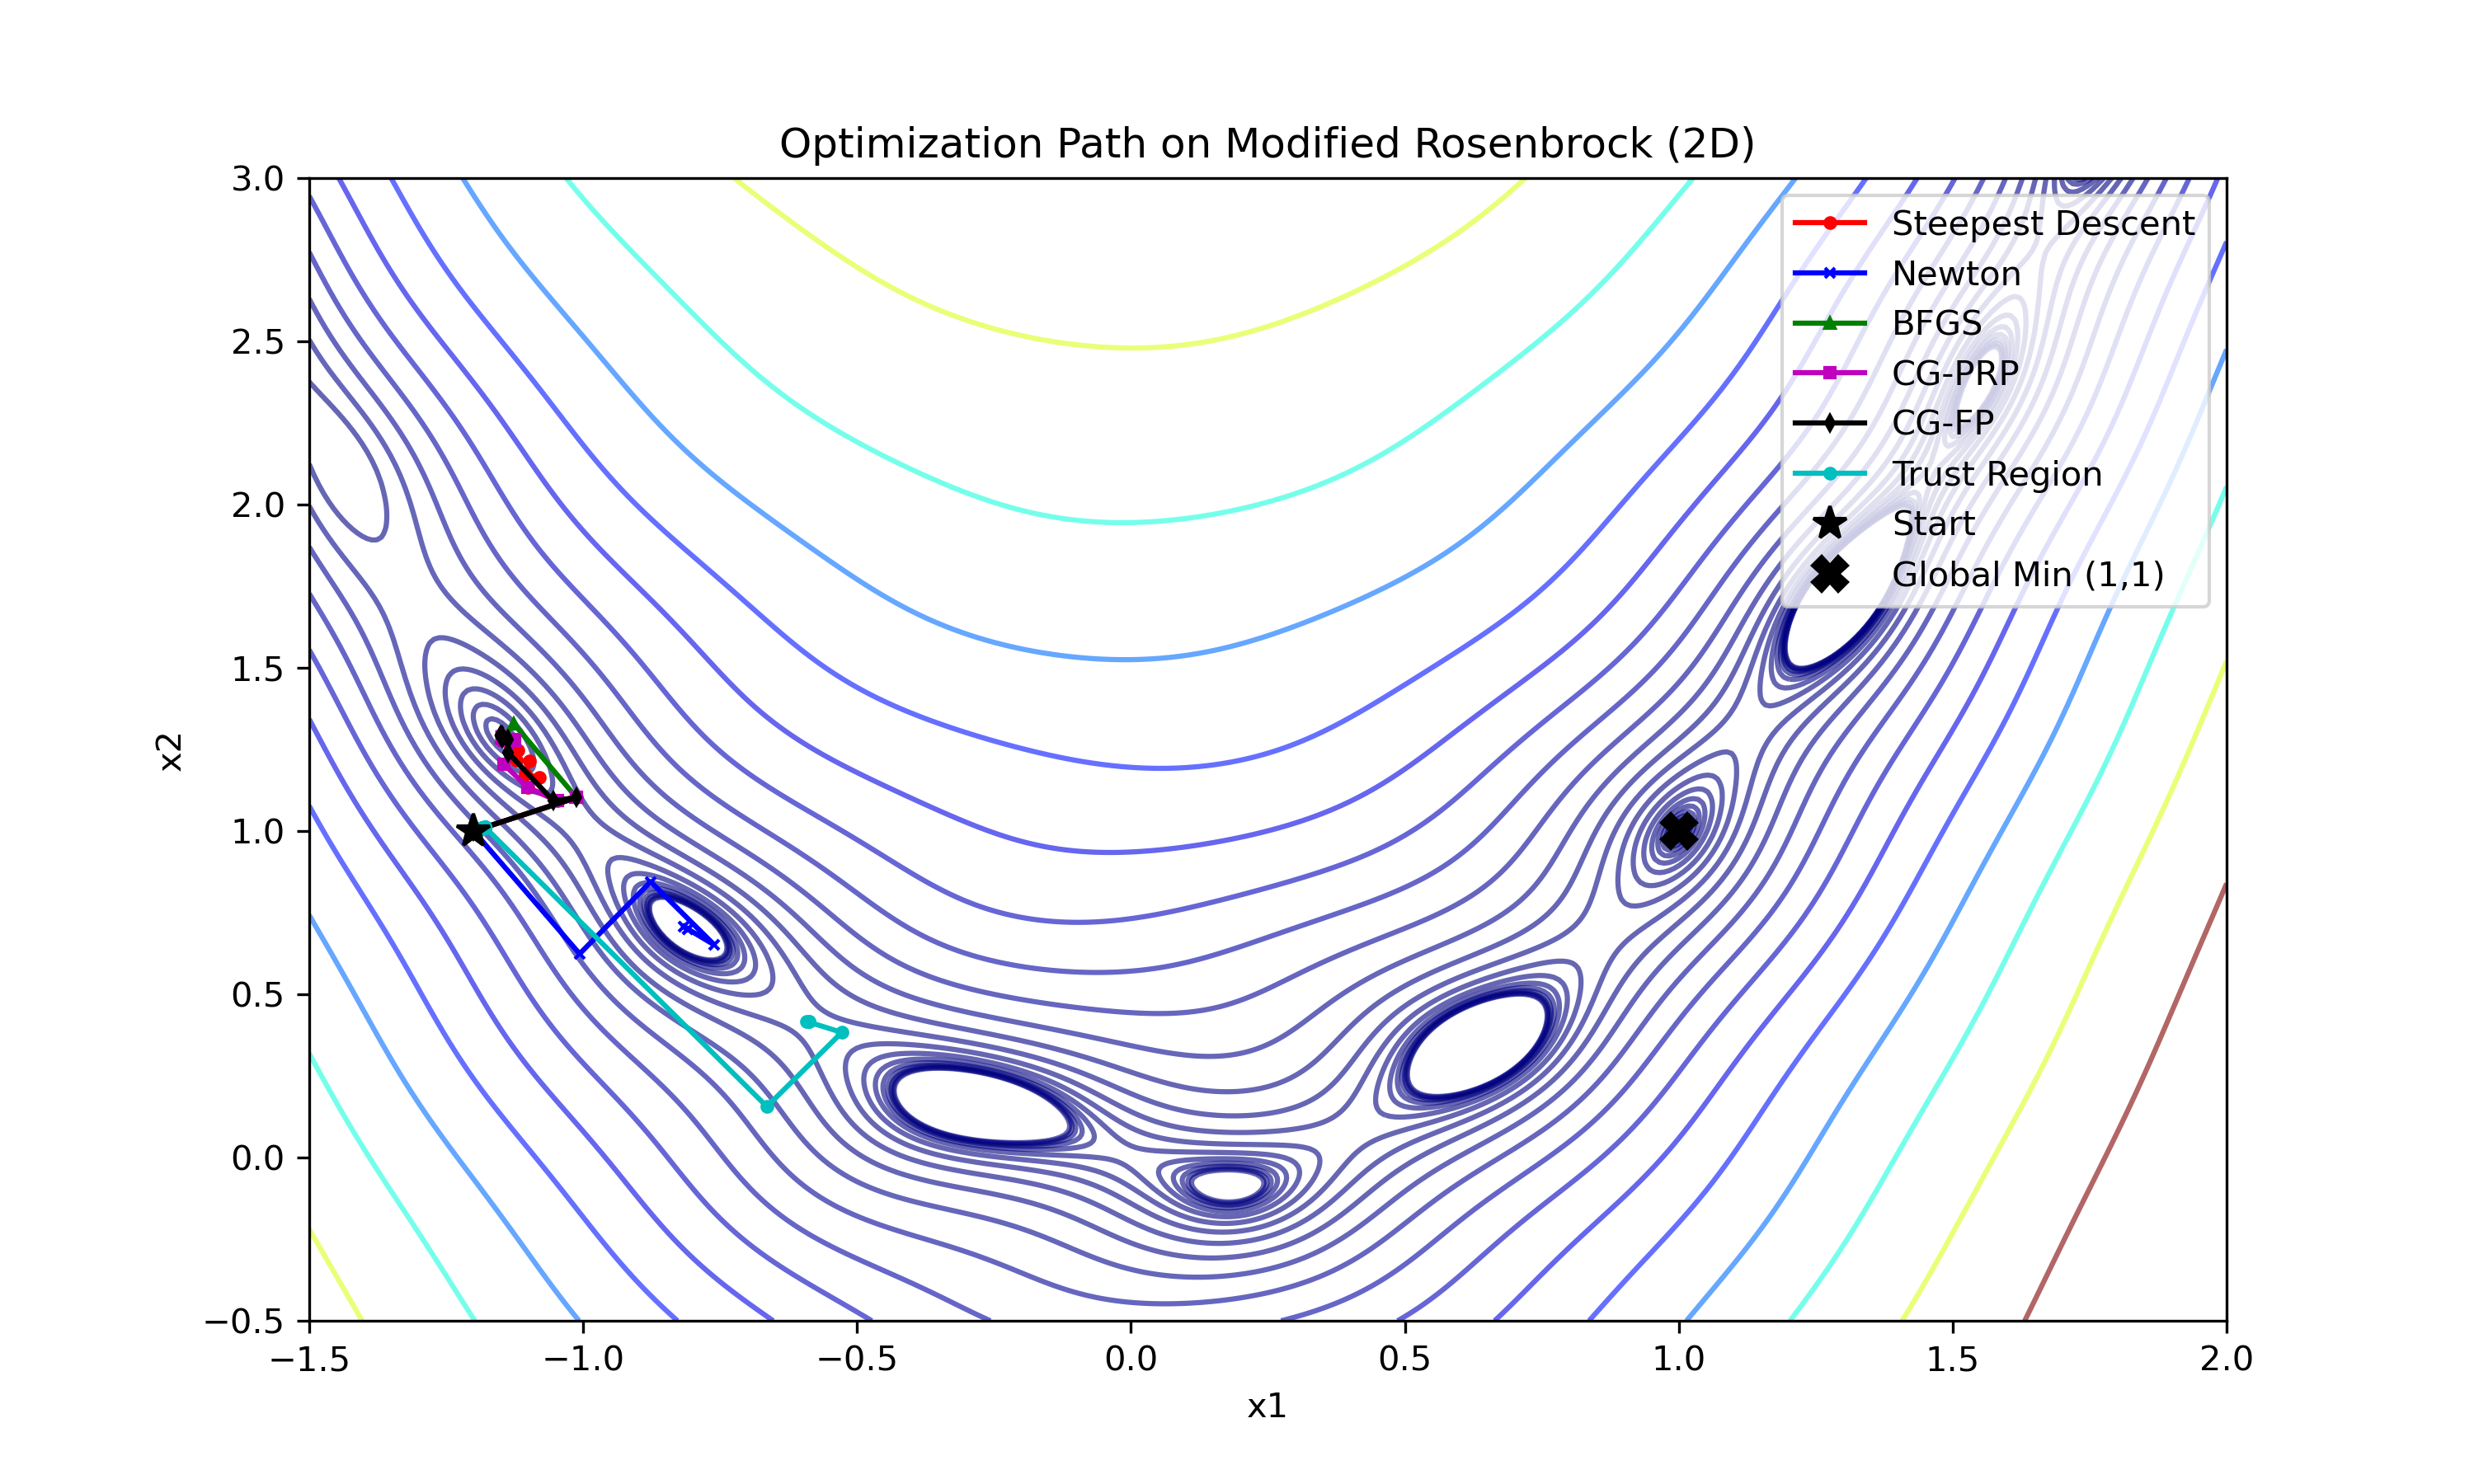
\includegraphics[width=0.8\textwidth]{optimization_paths_2d_inexact.png}}
    \\ 
    \subfloat[2D Modified Rosenbrock 优化路径 (Exact Search)]{
        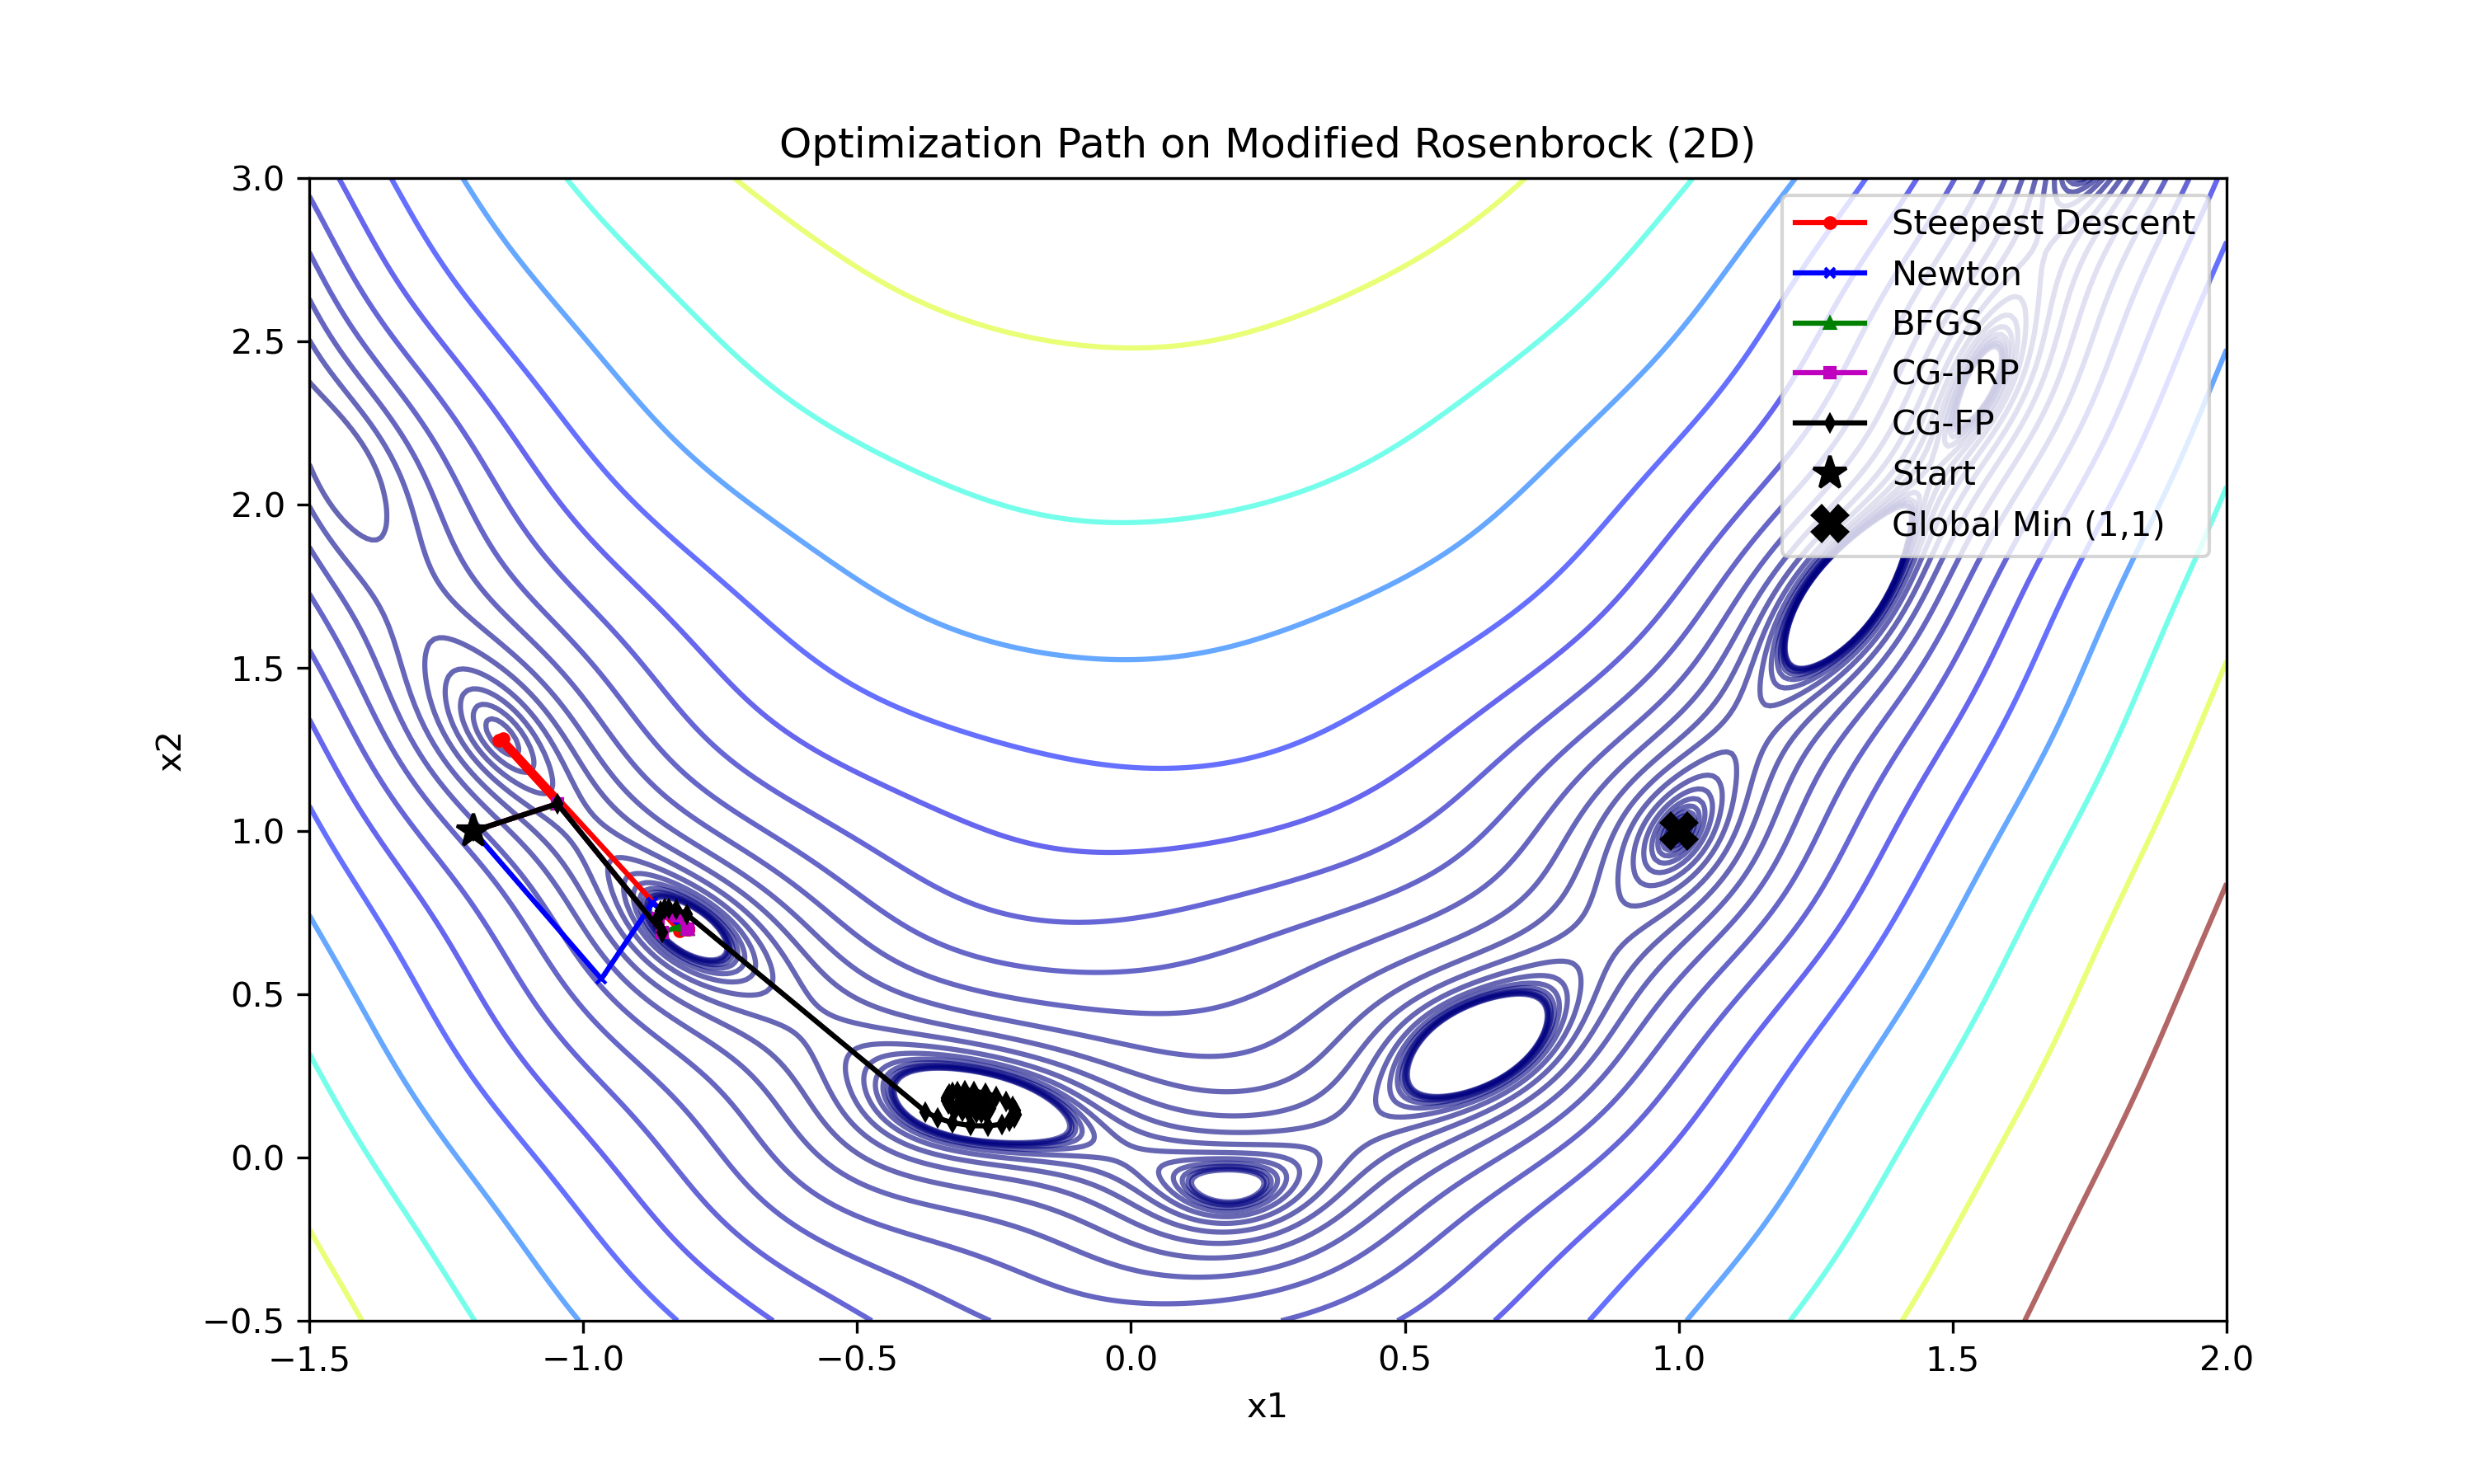
\includegraphics[width=0.8\textwidth]{optimization_paths_2d_exact.png}}
    \caption{各算法优化路径对比}
    \label{fig:opt_paths}
\end{figure}
\paragraph{非精确线搜索与信赖域算法的表现（子图a）}
在采用 Armijo+Wolfe 非精确线搜索策略时，算法表现出明显的“短视”特征。由于非精确搜索仅要求目标函数值有一定程度的下降（Sufficient Decrease），算法极易被路径上的第一个局部坑洼捕获。从图中可以看出，最速下降法（红线）、BFGS（绿线）和 CG-PRP（紫线）几乎在起步阶段就停止了更新，陷入了离初始点最近的微小凹陷中。相比之下，牛顿法（蓝线）和信赖域算法（青线，TR）利用二阶曲率信息尝试了大步长的跳跃，成功跨越了初始的若干障碍，深入到了山谷底部（$x \approx -0.8$ 和 $x \approx -0.5$ 附近）。然而，由于信赖域的半径限制以及正弦波导致的局部非凸性，它们最终也停滞在了半途的局部极小值处，无法翻越随后的山脊。这表明在多模态地形中，非精确搜索和信赖域策略倾向于快速收敛至最近的稳定点，缺乏跳出局部最优的能力。

\paragraph{精确线搜索的表现（子图b）}
当采用精确线搜索策略时，部分算法的搜索轨迹发生了显著变化，其中最引人注目的是 CG-FP 算法（黑线）。与非精确搜索相比，精确搜索要求在搜索方向上找到真正的极小值点。这种策略使得算法在面对地形上的微小波纹时，具有一定的“跨越”能力——即如果搜索方向延伸处的远处有一个更深的低谷，精确搜索会引导算法跳过中间较浅的局部坑洼。图中黑线（CG-FP）展现了剧烈的锯齿状行进路线，并成功比其他算法走得更远，到达了 $x \approx -0.3$ 附近的区域。然而，即便是精确搜索也无法改变梯度下降类算法的局部搜索本质，牛顿法（蓝线）和 BFGS（绿线）依然受困于早期的局部盆地中。这进一步验证了 Modified Rosenbrock 函数的复杂性：从该初始点出发，不存在一条单调下降的路径通往全局最优解，任何基于梯度的确定性算法在此处都面临失效风险。

\subsection{算法综合性能总结}

基于本次实验对 2D 多模态函数和 4D 高维病态函数的测试结果，对各优化算法的性能总结如下：

\begin{itemize}
    \item \textbf{线搜索策略 (Exact vs. Inexact)：} 
    虽然精确线搜索 (Exact) 理论上每步下降量最大，通常能减少迭代次数。但在复杂的 4D 地形中，非精确线搜索 (Armijo+Wolfe) 有时反而更具优势（如 4D Newton 中 Inexact 9次 < Exact 11次）。这是因为适当的“不精确”能避免算法过度拟合局部的微小弯曲，反而有助于更平滑地逼近极值点。考虑到计算成本，\textbf{非精确线搜索}在工程实现中性价比更高。

    \item \textbf{最速下降法 (Steepest Descent)：} 
    该算法结构简单，单步计算代价低。然而，由于仅利用一阶梯度信息，其收敛速度呈线性。实验表明，在\textbf{病态 (Ill-conditioned)} 的 4D Rosenbrock 问题中，该算法极易产生“锯齿现象”而停滞不前，完全无法在规定迭代次数内收敛。因此，它仅适用于良态问题或对解的精度要求不高的场景。

    \item \textbf{牛顿法 (Newton's Method)：} 
    该算法利用海森矩阵 (Hessian) 的二阶信息，具备\textbf{二次收敛速度}，在接近极值点时效率极高（通常 $<20$ 次迭代）。其局限性在于计算成本昂贵（需计算 Hessian 及其逆矩阵），且鲁棒性较差。实验中在 2D 函数特定初值下的发散现象，证实了其对 Hessian 矩阵正定性的敏感依赖。

    \item \textbf{BFGS 拟牛顿法：} 
    \textbf{综合性能最佳}。BFGS 成功结合了最速下降法的稳健性与牛顿法的快收敛性。它通过迭代更新近似矩阵避免了直接计算 Hessian，同时保持了超线性收敛速率。实验数据证明，无论是在多模态的 2D 问题还是高维病态的 4D 问题中，BFGS 均表现出极高的鲁棒性和优越的收敛率，是解决无约束优化问题的首选算法。

    \item \textbf{共轭梯度法 (Conjugate Gradient, CG)：}
    性能介于最速下降法和拟牛顿法之间。它克服了最速下降法的锯齿问题，在 4D 病态问题中能够收敛，且存储需求极低（无需存储矩阵）。然而，实验显示其性能对\textbf{线搜索精度}和\textbf{更新公式}高度敏感：PRP 公式在非精确搜索下表现较稳健，而 FP 公式在复杂地形下容易出现震荡或发散（如收敛曲线所示）。


    \item \textbf{信赖域算法 (Trust Region)：}
    尽管理论上具有较强的全局收敛性，但在本次实验的特定参数设置下，其表现不如线搜索类的二阶方法。特别是在 Modified Rosenbrock 的多模态地形中，由于局部二次模型（Quadratic Model）无法准确拟合叠加了高频正弦波的复杂曲面，导致信赖域半径被反复缩小，造成迭代停滞或陷入非最优的局部极小值。

\end{itemize}

\section{思考题}

\subsection{为什么牛顿法在二次函数上能“一步收敛”，而最速下降法需要多次迭代？}
\textbf{答：} 
对于二次函数 $f(\bm{x}) = \frac{1}{2}\bm{x}^T \bm{Q} \bm{x} + \bm{b}^T \bm{x} + c$，其梯度为 $\nabla f(\bm{x}) = \bm{Q}\bm{x} + \bm{b}$，Hessian 矩阵为常数阵 $\nabla^2 f(\bm{x}) = \bm{Q}$。
牛顿法的迭代公式为 $\bm{x}_{k+1} =\bm{x}_k - \bm{Q}^{-1}\nabla f(x)= \bm{x}_k - \bm{Q}^{-1}(\bm{Q}\bm{x}_k + \bm{b})$。整理可知 $\bm{x}_{k+1} = -\bm{Q}^{-1}\bm{b}$，这正是二次函数的极值点解析解。因此，无论初始点在哪，牛顿法利用了精确的二阶曲率信息，一步即可到达最优解。相较之下，最速下降法仅利用负梯度方向 $-\nabla f(\bm{x})$，只知道当前的下降方向，而不知道极小值有多远。。在二次函数等高线为椭球（$\bm{Q}$ 的特征值差异大，即条件数大）的情况下，负梯度方向与指向圆心的方向存在偏差。算法会沿着椭球的长轴和短轴反复震荡（Zig-zag），每次迭代只能消除一个方向的误差，因此收敛速度仅为线性，且受条件数影响严重。

\subsection{BFGS 拟牛顿法无需直接计算 Hessian 矩阵，却能达到接近牛顿法的收敛速度，其核心思想是什么？}
\textbf{答：}
其核心思想是\textbf{“曲率信息的积累与近似”}。BFGS 不直接计算海森矩阵，而是维护一个近似矩阵 $B_k$（或其逆 $H_k$）。在每次迭代中，利用梯度的变化量 $y_k$ 和位移量 $s_k$，通过秩2修正公式更新这个矩阵，使其满足拟牛顿条件 $H_{k+1} y_k = s_k$。
随着迭代进行，这个矩阵逐渐逼近真实的 Hessian 矩阵（或其逆），从而使搜索方向逐渐具备了牛顿方向的性质。因此，BFGS 能够在避免 $O(n^3)$ 的求逆运算和二阶导数计算代价的同时，获得超线性的收敛速度。

\subsection{共轭梯度法在非二次函数上的收敛性能为何不如 BFGS？这与“共轭方向”的性质有何关系？}
\textbf{答：}
共轭梯度法 (CG) 的收敛理论是建立在严格凸二次函数基础上的，其搜索方向关于常数 Hessian 矩阵 $\bm{Q}$ 共轭。而在一般非二次（非线性）函数优化中，CG 的性能往往不如 BFGS，主要原因归纳如下：

\begin{itemize}
    \item \textbf{共轭性的破坏：} 
    “共轭方向”的定义严格依赖于 Hessian 矩阵。在二次函数中，Hessian 矩阵 $\bm{Q}$ 是常数，共轭性始终保持。
    在非二次函数中，Hessian 矩阵 $\nabla^2 f(\bm{x})$ 随迭代点位置 $\bm{x}$ 实时变化。CG 算法基于前一步信息构造出的“共轭方向”，是关于“旧的”Hessian 共轭，而对于“当前”的 Hessian 往往不再共轭。
    这意味着 CG 在迭代过程中容易丢失共轭性质，导致算法退化为类似最速下降法的锯齿状搜索，收敛效率大幅降低。
    \item \textbf{信息利用率的差异：}
    共轭梯度法（CG）是一种“这一步算完就忘”的方法。它仅利用当前梯度和上一步的方向来构造新方向，虽然存储需求极低（$O(n)$），但缺乏对历史曲率信息的长期记忆。
    而BFGS显式地维护一个 $n \times n$ 的矩阵来逼近 Hessian 的逆。它能够持续积累和更新历史迭代中的曲率信息。在面临如 Rosenbrock 函数这种非二次性很强（弯曲峡谷）的问题时，BFGS 的“全局记忆”使其能更好地适应剧烈的地形变化。
    \item \textbf{重置策略：}
    由于共轭性的失效，CG 在非线性问题中通常需要频繁“重启”（如本实验采用的 PRP 策略，重置为负梯度方向）以避免搜索方向失效，且 CG 对线搜索的精度要求较高。相比之下，BFGS 对非精确线搜索（Inexact Line Search）和病态问题具有更强的鲁棒性，表现更为稳健。
\end{itemize}

\end{document}